\ifx\wholebook\relax \else

\documentclass{article}

\usepackage[nomarginpar
  %, margin=.5in
]{geometry}

\addtolength{\oddsidemargin}{-0.05in}
\addtolength{\evensidemargin}{-0.05in}
\addtolength{\textwidth}{0.1in}

\usepackage[en]{../prelude}

\setcounter{page}{1}

\begin{document}

\title{Infinity}

\author{Liu Xinyu
\thanks{{\bfseries Liu Xinyu} \newline
  Email: liuxinyu95@gmail.com \newline}
  }

\maketitle
\fi

\markboth{Infinity}{Mathematics of Programming}

\ifx\wholebook\relax
\chapter{Infinity}
\numberwithin{Exercise}{chapter}
\fi

\epigraph{I see it, but I don't believe it.}{ —— Georg Cantor, in a letter to Dedekind in 1877}

% "I see it, but I don't believe it." -- Richard Dedekind

\begin{wrapfigure}{R}{0.5\textwidth}
 \centering
 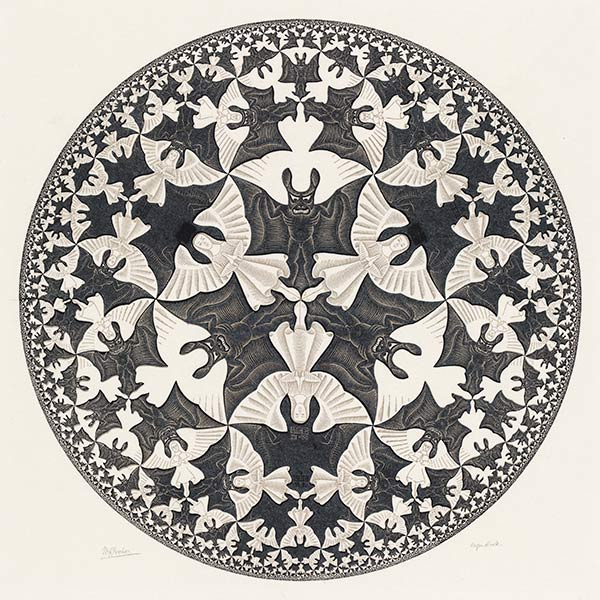
\includegraphics[scale=0.3]{img/circle-limit-IV-1960.eps}
 \captionsetup{labelformat=empty}
 \caption{Escher, Circle limit IV (Heaven and Hell), 1960}
 \label{fig:Circle-Limit-IV}
\end{wrapfigure}

Long time ago, our ancestor looked up at the starry sky, facing the vast galaxy, and came up with such a question, how big is the world we live in? As the intelligence being, our mind exceeds ourselves, exceeds our planet and universe. We keep thinking about the concept of infinity. People first abstracted numbers from concrete things. From the three goats hunted, three fruits collected, three jars made, obtained the abstract number three to represents any three things. At the beginning, the numbers were not big, that satisfied everyday life, hunting, and work. As the civilization evolved, people started trading things. People developed varies numbering system to support the bigger and bigger numbers. At some time point, we came up with the question: what is the biggest number? There were two different opinions to it. Some people didn't think the question make sense. It's enough to master numbers like thousands or millions in ancient time in everyday work and life. We needn't trouble ourselves with the big numbers that never being used. It's safe to consider the number of sand-grains in the world is infinity. In ancient Greece, people thought then thousands was a very big number, and named it `murias'. It finally changed to `myriad', means infinity\cite{De-linfini-2018}. In Buddhism, people also said the sand in Ganges River to indicate the numbers that are too large to count. In the Mahayana Buddhist classic work {\em The Diamond Sutra}, it said: ``If a virtuous man or woman filled a number of universes, as great as the number of sand-grains in all these rivers, with the seven treasures, and gave them all away in alms (dana), would his or her merit be great?'' Other people had different opinion. The great ancient Greek mathematician, Archimedes believed, even the sands-grains that filled the whole universe, can be represented with a definite number. In his book, {\em The Sand-Reckoner}, Archimedes said:

\begin{quotation}
\itshape
THERE are some, King Gelon, who think that the number of the sand is infinite in multitude; and I mean by the sand not only that which exists about Syracuse and the rest of Sicily but also that which is found in every region whether inhabited or uninhabited. Again there are some who, without regarding it as infinite, yet think that no number has been named which is great enough to exceed its multitude. And it is clear that they who hold this view, if they imagined a mass made up of sand in other respects as large as the mass of the earth, including in it all the seas and the hollows of the earth filled up to a height equal to that of the highest of the mountains, would be many times further still from recognising that any number could be expressed which exceeded the multitude of the sand so taken. But I will try to show you by means of geometrical proofs, which you will be able to follow, that, of the numbers named by me and given in the work which I sent to Zeuxippus, some exceed not only the number of the mass of sand equal in magnitude to the earth filled up in the way described, but also that of a mass equal in magnitude to the universe.
\end{quotation}

\begin{figure}[htbp]
%\begin{wrapfigure}{R}{0.4\textwidth}
 \centering
 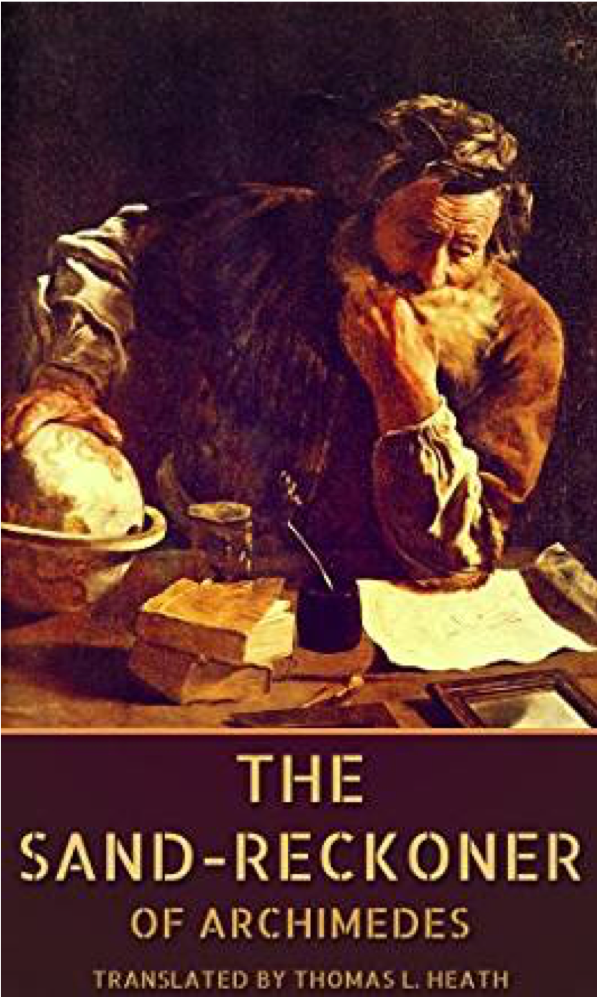
\includegraphics[scale=0.5]{img/Archimedes.eps}
 \captionsetup{labelformat=empty}
 \caption{The cover of {\em The Sand-Recokoner}. Archimedes Thoughtful by Domenico Fetti (1620)}
 \label{fig:Archimedes}
%\end{wrapfigure}
\end{figure}

Archimedes thought it {\em only} need $10^{63}$ sand-grains to fill the universe. The universe he meant was the sphere of the fixed star, which was about twenty thousands times the radius of the earth. We know the observable universe is about 46.5 billion light-years nowadays, consist of around $3 \times 10^{74}$ atoms\footnote{Also said to have $10^{80}$ to $10^{87}$ elementary particles.}. Archimedes was definitely genius in ancient Greek time, he demonstrated how to quantify the `infinite big' things. There are many words in different languages serve as the unit for big numbers. The following table list these words in Chinese, they increase for every $10^4$(\cite{Noguchi2007}, pp31).

\begin{center}
% for Pinyin tones: \={a}, \'{a}, \v{}, \.{a}
\begin{tabular}{|l|r|l|r|}
\hline
{\fontspec{\cnmainft}京}            & $10^{16}$ & {\fontspec{\cnmainft}载}            & $10^{44}$ \\
\hline
{\fontspec{\cnmainft}垓}(g\={a}i)   & $10^{20}$ & {\fontspec{\cnmainft}极}            & $10^{48}$ \\
\hline
{\fontspec{\cnmainft}秭}(z\v{i})    & $10^{24}$ & {\fontspec{\cnboldft}恒河沙}  & $10^{52}$ \\
\hline
{\fontspec{\cnmainft}穰}(r\'{a}ng)  & $10^{28}$ & {\fontspec{\cnmainft}阿僧祗}(zh\={i})  & $10^{56}$ \\
\hline
{\fontspec{\cnmainft}沟}            & $10^{32}$ & {\fontspec{\cnmainft}那由他}        & $10^{60}$ \\
\hline
{\fontspec{\cnmainft}涧}            & $10^{36}$ & {\fontspec{\cnmainft}不可思议}      & $10^{64}$ \\
\hline
{\fontspec{\cnmainft}正}            & $10^{40}$ & {\fontspec{\cnmainft}无量大数}      & $10^{68}$ \\
\hline
\end{tabular}
\end{center}

Many such words come from Buddhism, like {\fontspec{\cnmainft}恒河沙}, means the sand-grain in Ganges River. It has 52 zeros after 1. Below table list the unit words in English. Start from one, there is a unit for every 1000 magnitude. Compare to 10000 magnitude step in Chinese, we can see the culture difference.

\begin{center}
\begin{tabular}{|l|r|l|r|l|r|}
\hline
thousand & $10^{3}$ & quattuordecillion & $10^{45}$ & octovigintillion & $10^{87}$ \\
\hline
million & $10^{6}$ & quindecillion & $10^{48}$ & novemvigintillion & $10^{90}$ \\
\hline
billion & $10^{9}$ & sexdecillion & $10^{51}$ & trigintillion & $10^{93}$ \\
\hline
trillion  & $10^{12}$ & septdecillion & $10^{54}$ & untrigintillion & $10^{96}$ \\
\hline
quadrillion  & $10^{15}$ & octodecillion & $10^{57}$ & duotrigintillion & $10^{99}$ \\
\hline
quintillion  & $10^{18}$ & novemdecillion & $10^{60}$ & \textbf{googol} & $10^{100}$ \\
\hline
sexillion    & $10^{21}$ & vigintillion & $10^{63}$ & & \\
\hline
septillion   & $10^{24}$ & unvigintillion & $10^{66}$ & & \\
\hline
octillion    & $10^{27}$ & duovigintillion & $10^{69}$ & & \\
\hline
noniliion  & $10^{30}$ & trevigintillion & $10^{72}$ & & \\
\hline
decillion  & $10^{33}$ & quattuorvigintillion & $10^{75}$ & & \\
\hline
undecillion   & $10^{36}$ & quinvigintillion & $10^{78}$ & & \\
\hline
duodecillion  & $10^{39}$ & sexvigintillion & $10^{81}$ & & \\
\hline
tredecillion  & $10^{42}$ & seprvigintillion & $10^{84}$ & & \\
\hline
\end{tabular}
\end{center}

The last unit, googol, was coined in 1920 by 9-year-old Milton Sirotta, nephew of U.S. mathematician Edward Kasner. It is written as the digit 1 followed by one hundred zeros. The famous internet company Google's name came from this word\cite{Wikipedia-Googol}.

\section{The infinity concept}
\index{Zeno} \index{Zeno's paradox}

The existence of infinity that beyond all concrete numbers is not only a mathematical question, but also a philosophical question. Infinity also lead to the concept of infinitesimal. The ancient Greek philosopher, Zeno of Elea thought of a set of problems about infinity. Some of them are preserved in Aristotle's {\em Physics}. Among them, four paradoxes are most famous.

\begin{figure}[htbp]
%\begin{wrapfigure}{R}{0.3\textwidth}
 \centering
 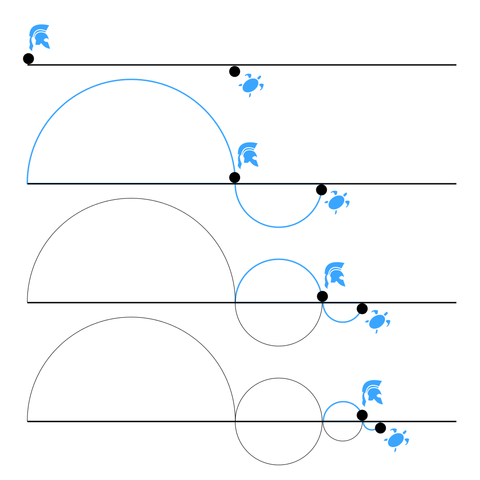
\includegraphics[scale=0.4]{img/Achilles-paradox.eps}
 %\captionsetup{labelformat=empty}
 \caption{Achilles and the tortoise}
 \label{fig:Achilles-paradox}
%\end{wrapfigure}
\end{figure}

The first one is the most popular, named Achilles and the tortoise paradox. Achilles In Greek mythology, Achilles was a hero of the Trojan War, the greatest of all the Greek warriors, and is the central character of Homer's {\em Iliad}. In this paradox, Achilles is in a footrace with the tortoise. Achilles allows the tortoise a head start of 100 meters, for example. Supposing that each racer starts running at some constant speed, one faster than the other. After some finite time, Achilles will have run 100 meters, bringing him to the tortoise's starting point. During this time, the tortoise has run a much shorter distance, say 2 meters. It will then take Achilles some further time to run that distance, by which time the tortoise will have advanced farther; and then more time still to reach this third point, while the tortoise moves ahead. Thus, whenever Achilles arrives somewhere the tortoise has been, he still has some distance to go before he can even reach the tortoise. as shown in figure \ref{fig:Achilles-paradox}. Although it contradicts our common sense in real life, the argument is so convincing. This paradox attracted many great minds for thousands of years. Lewis Carrol, and Douglas Hofstadter even took Achilles and the tortoise as figures in their literary works.

\begin{figure}[htbp]
%\begin{wrapfigure}{R}{0.3\textwidth}
 \centering
 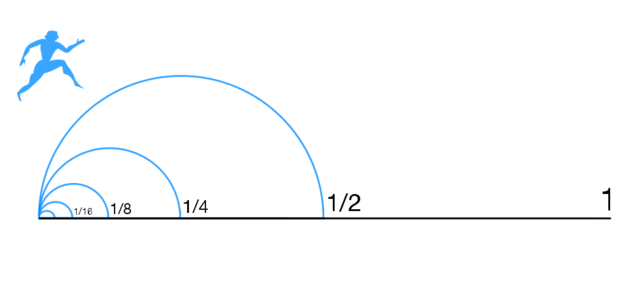
\includegraphics[scale=0.4]{img/Dichotomy-paradox.eps}
 %\captionsetup{labelformat=empty}
 \caption{Dichotomy paradox}
 \label{fig:Dichotomy-paradox}
%\end{wrapfigure}
\end{figure}

The second one is called Dichotomy paradox. Atalanta is a character in Greek mythology, a virgin huntress. Suppose Atalanta wishes to walk to the end of a path. Before she can get there, she must get halfway there. Before she can get halfway there, she must get a quarter of the way there. Before traveling a quarter, she must travel one-eighth; before an eighth, one-sixteenth; and so on. This description requires one to complete an infinite number of tasks, which Zeno maintains is an impossibility. The paradoxical conclusion then would be that travel over any finite distance can neither be completed nor begun, and so all motion must be an illusion.

The third one is called Arrow paradox. Zeno states that for motion to occur, an object must change the position which it occupies. He gives an example of an arrow in flight. He states that in any one (duration-less) instant of time, the arrow is neither moving to where it is, nor to where it is not. It cannot move to where it is not, because no time elapses for it to move there; it cannot move to where it is, because it is already there. In other words, at every instant of time there is no motion occurring. If everything is motionless at every instant, and time is entirely composed of instants, then motion is impossible. Whereas the first two paradoxes divide space, this paradox starts by dividing time—and not into segments, but into points.

\begin{figure}[htbp]
%\begin{wrapfigure}{R}{0.3\textwidth}
 \centering
 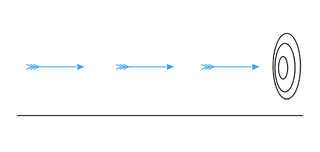
\includegraphics[scale=0.4]{img/Arrow-paradox.eps}
 \caption{Arrow paradox}
 \label{fig:Arrow-paradox}
\end{figure}

The fourth one is called the moving rows paradox, or stadium paradox. It also about dividing time into atomic points. As shown in figure \ref{fig:Moving-rows-paradox}, there are three rows in the stadium. Each row being composed of an equal number of bodies of equal size. At the beginning, they are all aligned. At the smallest time duration, row A stays, row B moves to the right one space unit, while row $\Gamma$ moves to the left one space unit. To row B, row $\Gamma$ actually moves two space units. It means, there should be time duration that $\Gamma$ moves one space unit relative to $B$. And it is the half time of the smallest duration. Since the smallest duration is atomic, it involves the conclusion that half a given time is equal to that time.

\begin{figure}[htbp]
 \centering
 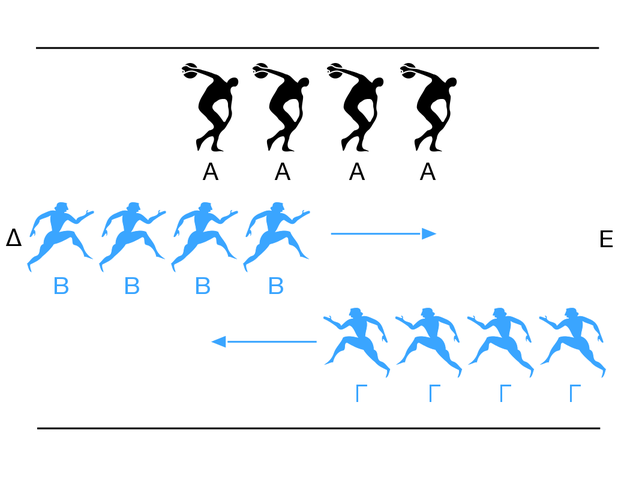
\includegraphics[scale=0.3]{img/Moving-rows-paradox.eps}
 \caption{Moving rows paradox}
 %\captionsetup{labelformat=empty}
 \label{fig:Moving-rows-paradox}
%\end{wrapfigure}
\end{figure}

Zeno's paradoxes are easy to understand. However, the conclusion is surprised. In our common sense, motion and time are so real. Achilles must be able to catch up the tortoise. It is hard to solve Zeno's paradox. From Aristotle to Bertrand Russel, from Archimedes to Herman Weyl, all proposed solutions to Zeno's paradoxes\cite{Wikipedia-Zeno}.

Zeno of Elea (about 490BC - 425BC) is ancient Greek philosopher.
He was born in Elea, which was a Greek colony located in present-day southern Italy. Little is known for certain about Zeno's life. In the dialogue of Parmenides, Plato describes a visit to Athens by Zeno and Parmenides, at a time when Parmenides is ``about 65'', Zeno is ``nearly 40'', and Socrates is ``a very young man''. Assuming an age for Socrates of around 20 and taking the date of Socrates' birth as 469 BC gives an approximate date of birth for Zeno of 490 BC. Some less reliable details of Zeno's life are given by Diogenes Laërtius in his {\em Lives and Opinions of Eminent Philosophers}. It said Zeno was the adopted son of Parmenides. He was skilled to argue both sides of any question, the universal critic. And that he was arrested and perhaps killed at the hands of a tyrant of Elea\cite{HanXueTao16}.

Zeno was the primary member of the Eleatics, which were a pre-Socratic school of philosophy founded by Parmenides in the early fifth century BC in the ancient town of Elea. It's another important school after Pythagoras. The Eleatics rejected the epistemological validity of sense experience, and instead took logical standards of clarity and necessity to be the criteria of truth. Of the members, Parmenides and Melissus built arguments starting from sound premises. Zeno, on the other hand, primarily employed the reductio ad absurdum, attempting to destroy the arguments of others by showing that their premises led to contradictions. Zeno is best known for his paradoxes, which Bertrand Russell described as ``immeasurably subtle and profound''.

\begin{figure}[htbp]
%\begin{wrapfigure}{L}{0.3\textwidth}
 \centering
 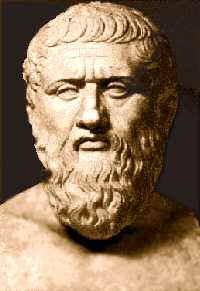
\includegraphics[scale=0.5]{img/Zeno.eps}
 \captionsetup{labelformat=empty}
 \caption{Zeno of Elea, About 490BC - 425BC}
 \label{fig:Zeno-of-Elea}
%\end{wrapfigure}
\end{figure}

Ancient Chinese philosophers developed equivalents to some of Zeno's paradoxes. From the surviving Mohist School of Names book of logic which states, in the archaic ancient Chinese script, ``a one-foot stick, every day take away half of it, in a myriad ages it will not be exhausted.''

Zeno's paradoxes caused deep confusion to the ancient Greeks. The views about time, space, infinity, continuity, and movement are critical to the later philosophers and mathematicians even today. How to understand infinity, became a problem that must be solved by ancient Greek philosophers.

\subsection{Potential infinity and actual infinity}
\index{potential infinity} \index{actual infinity}

Aristotle studied Zeno's paradoxes deeply (most of our understanding to Zeno's paradoxes is through Aristotle's {\em Physics}). One of the most important contributions that Aristotle had made to to study of infinity is identifying a dichotomy between what Aristotle calls the {\em potential infinite} and the {\em actual infinite}. This work fundamentally influenced the later development of mathematics\cite{HanXueTao16}. Potential infinity is a process that never stops. It can be a group of numbers or group of ``things'' that continues without terminating, going on or repeating itself over and over again with no recognizable ending point. The obvious example is the the grouping of natural numbers. No matter where you are while listing or counting out natural numbers, there always exists another number to proceed the one before. Also, in Euclid geometry, a line with a starting point could extend on without end, but could still be potentially infinite because all one would have to do is add on more length to a finite length to allow it to extend\footnote{Euclid avoided to use the term `infinitely extend' in his work. instead he said a line can be extended any long as needed. This is a common treatment in ancient Greece.}. The actual infinite involves  never-ending sets or ``things'' within a space that has a beginning and end; it is a series that is technically ``completed'' but consists of an infinite number of members. According to Aristotle, actual infinities cannot exist because they are paradoxical. It is impossible to say that you can always ``take another step'' or ``add another member'' in a completed set with a beginning and end, unlike a potential infinite. It is ultimately Aristotle’s rejection of the actual infinite that allowed him to refute Zeno’s paradox.

Although Aristotle did disprove the existence of the actual infinite finally, and tended to reject a lot of major concepts in mathematics, the importance of mathematics was still never belittled in Aristotle’s eyes. Aristotle argued that actual infinity as it is not applicable to geometry and the universal, is not relevant to mathematics, making potential infinity all that actually is important.

Aristotle's viewpoint to infinity is typical in ancient Greece. The dichotomy and controversy about potential infinity and actual infinity have been influential till today. Despite of these arguments, the ancient Greek mathematicians achieved amazing result with the potential infinity concept. On success story was that Euclid proved there are infinitely many prime numbers. It is considered the one of most beautiful proofs in history.

\begin{proposition}[Euclid's Elements, Book IX, Proposition 20]
Prime numbers are more than any assigned multitude of prime numbers\cite{Elements}.
\end{proposition}

Euclid intentional avoided using term like `infinitely many' when state this proposition. Such treatment is very common in his Elements. It's famous that Euclid uses reduction to absurdity in his proof. We explain it in modern language.

\begin{proof}
Suppose there are finite prime numbers $p_1, p_2, ..., p_n$. Euclid makes a new number:

\[
p_1 p_2 ... p_n + 1
\]

Which is the product of the $n$ prime numbers plus one. It is either prime or not.

\begin{itemize}
\item If it is prime, definitely, it does not equal to any one from $p_1$ to $p_n$, hence it's a new prime not in the list;
\item If it is not prime, then it must have a prime factor $p$. However, no one from $p_1$ to $p_n$ divides this number. It means $p$ is different from any one from $p_1$ to $p_n$, hence it's a new prime beyond those in the list.
\end{itemize}

In both cases, we obtain a new prime number. It contradicts the assumption that there are finite prime numbers. Therefore, there are infinitely many prime numbers.
\end{proof}

From the view point today, Euclid obtained a kind of indirect `proof of existence'. By using proof by contradiction, he proved there are infinitely many prime numbers, but did not give the way to list them. It is quite natural in mathematical proofs now. However, it led to hotly debating about the fundamentals of mathematics in the late 19th and early 20th Century. We'll return to this topic in next chapter.

\begin{figure}[htbp]
%\begin{wrapfigure}{L}{0.3\textwidth}
 \centering
 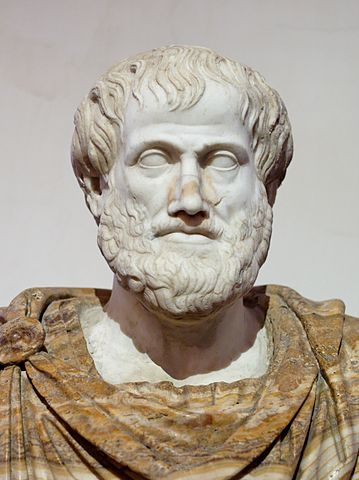
\includegraphics[scale=1]{img/Aristotle.eps}
 \captionsetup{labelformat=empty}
 \caption{Aristotle, 384BC - 322BC}
 \label{fig:Aristotle}
%\end{wrapfigure}
\end{figure}

\index{Aristotle}
Aristotle was a great philosopher and polymath in ancient Greece. Along with his teacher Plato, he has been called the `Father of Western Philosophy'. Little is known about his life. Aristotle was born in the city of Stagira in Northern Greece in 384BC. His father died when Aristotle was a child, and he was brought up by a guardian. At the age of seventeen or eighteen, he joined Plato's Academy in Athens and remained there for 20 years until Plato died. This period of study in Plato's Academy deeply influenced Aristotle's life. Socrates was Plato's teacher, and Aristotle was taught by Plato. He soon became an outstanding, and Plato called him ``the Spirit of the Academy''. But Aristotle is not a man who only admires authority without his own opinions. He studied hard, and even established a library for himself.

Shortly after Plato died around 347BC, Aristotle left Athens. The traditional story about his departure records that he was disappointed with the Academy's direction after control passed to Plato's nephew. After that, he traveled around. In 343 BC, Aristotle was invited by Philip II of Macedon to become the tutor to his 13 years old son Alexander. Aristotle was appointed as the head of the royal academy of Macedon. During Aristotle's time in the Macedonian court, he gave lessons not only to Alexander, but also to two other future kings: Ptolemy and Cassander. It was under the influence of Aristotle that Alexander the Great cared about science and respected knowledge.

In 335BC, Philip II died. Aristotle returned to Athens, establishing his own school there known as the Lyceum. Aristotle conducted courses at the school for the next twelve years. This period in Athens, between 335 and 323 BC, is when Aristotle is believed to have composed many of his works. He studied and made significant contributions to ``logic, metaphysics, mathematics, physics, biology, botany, ethics, politics, agriculture, medicine, dance and theatre.'' There was legend that Aristotle had a habit of walking while lecturing along the walkways covered with colonnades. It was for this reason that his school was named ``Peripatetic'' (an ancient Greek word, which means ``of walking'' or ``given to walking about''). Aristotle used the language that was much more obscure than Plato's Dialogue. Many of his works are based on lecture notes, and some are even the notes of his students. Aristotle was considered for the first author of textbooks in the West World.

Following Alexander's death, anti-Macedonian sentiment in Athens was rekindled. In 322 BC, his enemies reportedly denounced Aristotle for impiety, prompting him to flee to his mother's family estate in Euboea, at which occasion he was said to have stated: ``I will not allow the Athenians to sin twice against philosophy'' – a reference to Athens's trial and execution of Socrates. He died on Euboea of natural causes later that same year, at the age of 63.

More than 2300 years after his death, Aristotle remains one of the most influential people who ever lived. He contributed to almost every field of human knowledge then in existence, and he was the founder of many new fields. Among countless other achievements, Aristotle was the founder of formal logic, pioneered the study of zoology, and left every future scientist and philosopher in his debt through his contributions to the scientific method.

\subsection{Method of exhaustion and calculus}
\index{method of exhaustion}

Some other ancient Greek mathematician took the practical approach about infinity. They developed the method of exhaustion and made surprising achievement.

The idea of method of exhaustion originated in the late 5th Century BC with Antiphon (About 480BC - 410BC). To solve one of the three classic geometric problems, square the circle\footnote{The other two are trisecting the angle, and doubling the cube. Given a circle, ancient Greeks attempted to seek the solution to draw a square that has the same area with only straightedge and compass. Many mathematicians attempted to solve this problem, but all failed until Galois developed theory to prove they were all impossible in 19th Century.}. To approximate the area of a circle, Antiphon started from an inscribed square, then repeatedly double the number of the sides to obtain octagons, hexagons... As the area of the circle gradually ``exhausts'', the side length of inscribed polygons gets smaller and smaller. Antiphon thought the polygon would eventually coincide with the circle. This is the idea of exhaustion. The method was made rigorous a few decades later by Eudoxus of Cnidus, who used it to calculate areas and volumes. The correctness of this method relies on the famous axiom of Eudoxus-Archimedes, also known as axiom of Archimedes.

\index{axiom of Archimedes}
\begin{axiom}
\normalfont
\textbf{Axiom of Archimedes} Given two magnitudes $a$ and $b$, there exists some natural number $n$, such that $a \leq nb$.
\end{axiom}

Axiom of Archimedes is fundamental. We introduced Euclid algorithm to compute the greatest common measurement in chapter 2, however, we did not show if this algorithm always terminates. With axiom of Archimedes, we can prove that Euclid algorithm always terminates. Eudoxus stated ``Given two different magnitudes, for the larger one, subtract a magnitude larger than its half, then for the remaining, subtract another magnitude larger than its half, repeat this process, there must be some remaining less than the smaller one.'' This is logic behind the method of exhaustion.

By using the method of exhaustion, Eudoxus proved that: the volume of a pyramid is one-third the volume of a prism with the same base and altitude, and the volume of a cone is one-third that of the corresponding cylinder. These statements are summarized as propositions in the book 12 of Euclid's {\em Elements}\cite{HanXueTao16}.

Archimedes greatly developed the method of exhaustion, and achieved the highest level, amazing result. He calculated $\pi$, proved the formulas of circular area, surface area and volume of sphere, cone, and even found the method to calculate the area under the parabola curve. He was said to be the god of the mathematics in ancient Greece.

%\begin{figure}[htbp]
\begin{wrapfigure}{R}{0.4\textwidth}
 \centering
 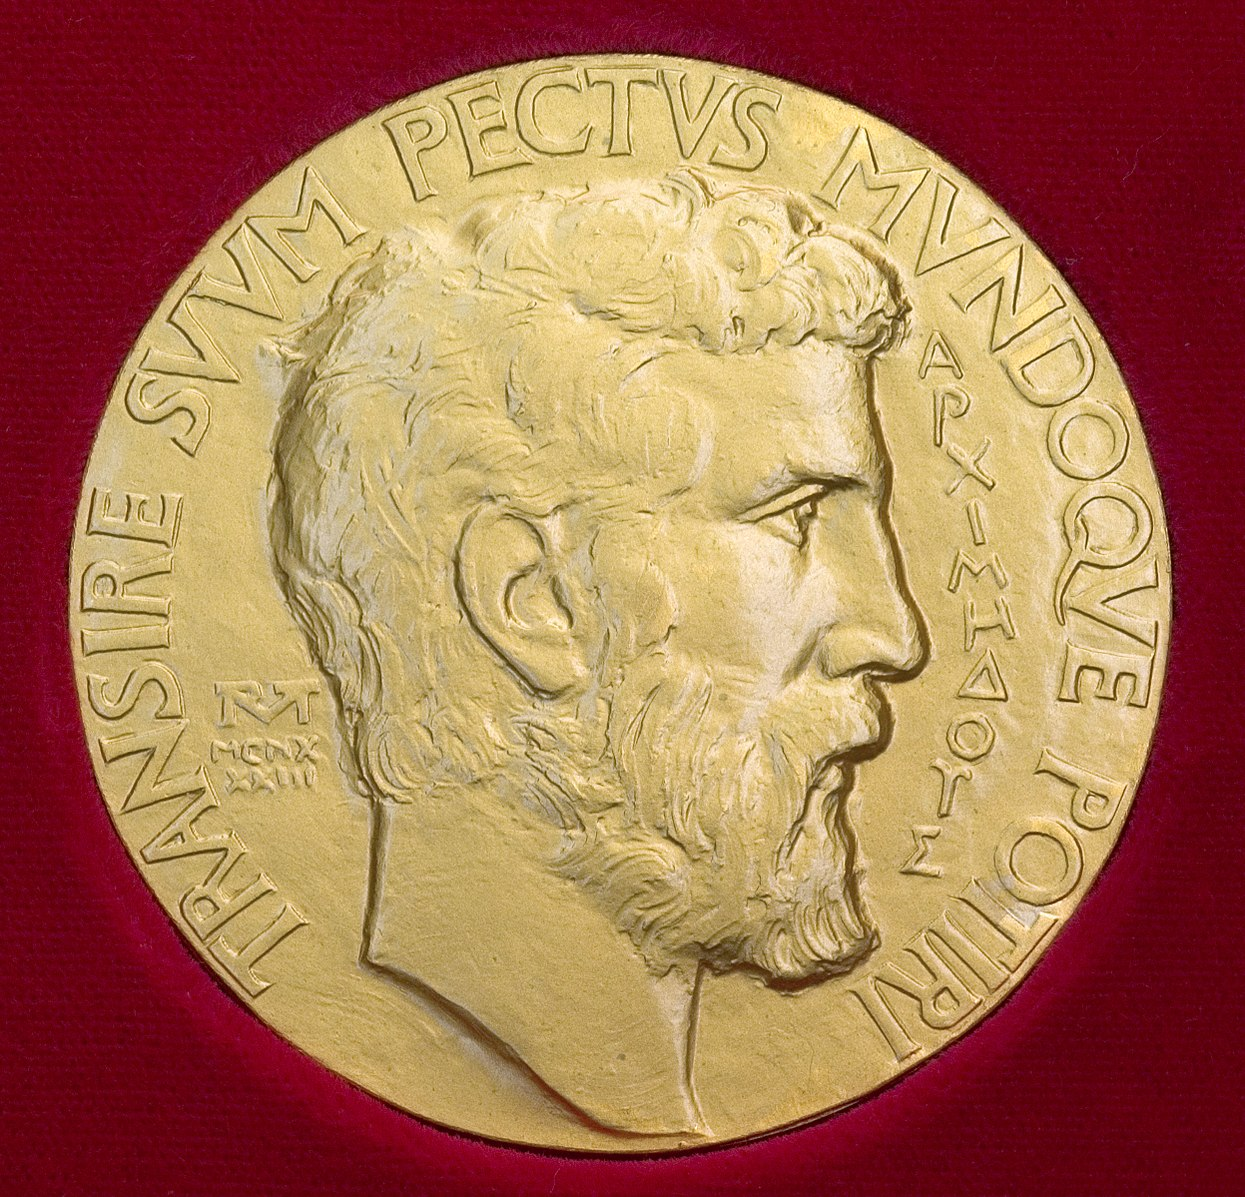
\includegraphics[scale=0.1]{img/FieldsMedal.jpg}
 \captionsetup{labelformat=empty}
 \caption{The Fields Medal carries a portrait of Archimedes.}
 \label{fig:FieldsMedal}
\end{wrapfigure}
%\end{figure}

\index{Archimedes}
Archimedes (287BC - 212 BC) was a Greek mathematician, physicist, engineer, inventor, and astronomer. He was bore in the seaport city of Syracuse, at that time a self-governing colony in Magna Graecia. During his youth, Archimedes may have studied in Alexandria, Egypt. During his lifetime, Archimedes made his work known through correspondence with the mathematicians in Alexandria. Although few details of his life are known, he is considered the greatest mathematician of antiquity and one of the greatest of all time. various stories about him are widely circulated and popular.

The most widely known anecdote about Archimedes tells of how he uncovered a fraud in the manufacture of a golden crown commissioned by King Hiero II of Syracuse. The king had supplied the pure gold to be used, and Archimedes was asked to determine whether some silver had been substituted by the dishonest goldsmith. Archimedes had to solve the problem without damaging the crown, so he could not melt it down into a regularly shaped body in order to calculate its density. While taking a bath, he noticed that the level of the water in the tub rose as he got in, and realized that this effect could be used to determine the volume of the crown. Archimedes then took to the streets naked, so excited by his discovery that he had forgotten to dress, yelling ``Eureka!'' (Greek word meaning ``I have found [it]!''). The test was conducted successfully, proving that silver had indeed been mixed in. His discovery is the ``Archimedes' Principle'' that every middle school student must learn. Eureka was later used to describe the moment when inspiration was found.

In 214BC, the Second Punic War Broke out. Legend has it that Archimedes created a giant parabolic mirror to deflect the powerful Mediterranean sun onto the ship's sails, setting fire to them. Archimedes also created a huge crane operated hook – the Claw of Archimedes – that was used to lift the enemy ships out of the sea before dropping them to their doom. After two-year-long siege, In 212 BC, the Romans captured Syracuse. The Roman force commander, Marcellus had ordered that Archimedes, the well-known mathematician should not be killed. Archimedes, who was now around 78 years of age, continued his studies after the breach by the Romans and while at home, his work was disturbed by a Roman soldier. The last words attributed to Archimedes are ``Do not disturb my circles!'' The soldier killed Archimedes despite orders that Archimedes should not be harmed. 137 years after his death, the Roman orator Cicero described visiting the tomb of Archimedes. It was surmounted by a sphere and a cylinder, which Archimedes had requested be placed on his tomb to represent his mathematical discoveries\footnote{A sphere has 2/3 the volume and surface area of its circumscribing cylinder including its bases.}.

% Sphere: 4/3 pi r^3, Cylinder: pi r^2 * 2r = 2 pi r^3
% ==> S : C = 4/3 / 2 = 2/3

As an example, let us see how Archimedes calculated $\pi$ with the method of exhaustion around 250BC. Symbol $\pi$ represents the ratio of a circle's circumference to its diameter, sometimes it's referred to as Archimedes' constant.

As shown in \ref{fig:pi-exhaustion}, Archimedes drew two regular polygons inside and outside a circle of diameter of 1. For a side of the inscribed polygon and the corresponding arc, the length of the arc is greater than the side because the straight line is the shortest between two points. Hence the circumference of the circle is greater than the inscribed polygon. Similarly, circumference of the circle is less than the circumscribed polygon. Since the diameter is 1, the circle's circumference equals $\pi$. Hence the below relation holds:

\[
  C_i < \pi < C_o
\]

\begin{figure}[htbp]
%\begin{wrapfigure}{R}{0.4\textwidth}
 \centering
 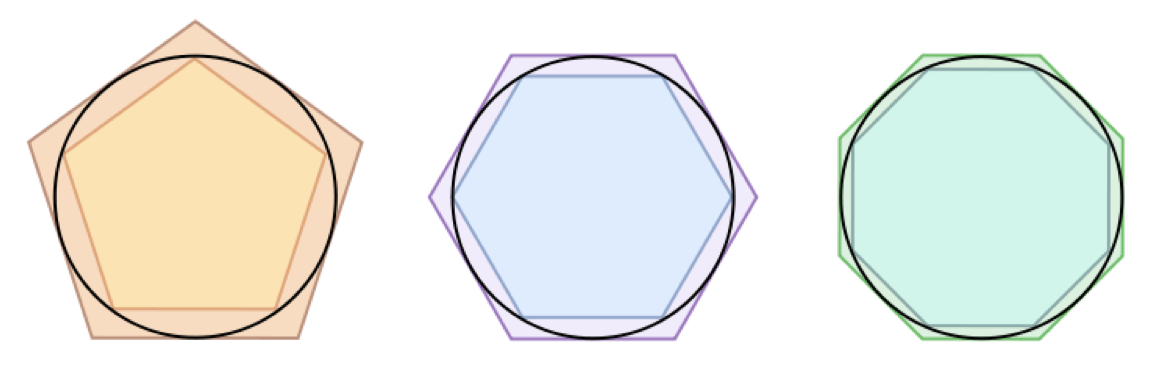
\includegraphics[scale=0.5]{img/pi-exhaustion.eps}
 %\captionsetup{labelformat=empty}
 \caption{π can be estimated by computing the perimeters of circumscribed and inscribed polygons.}
 \label{fig:pi-exhaustion}
%\end{wrapfigure}
\end{figure}

Where $C_i$ and $C_o$ are the circumferences of the inscribed and circumscribed polygons respectively. Successively increasing the number of sides approximates the range of $\pi$. Archimedes calculated the 96-sided regular polygon, he proved that $\dfrac{223}{71} < \pi < \dfrac{22}{7}$ (that is $3.1408 < \pi < 3.1429$). This upper bound of $\dfrac{22}{7}$ is widely used in western. The Chinese mathematician Zu Chongzhi, around 480AD, calculated that $3.1415926 < \pi < 3.1415927$ and suggested the approximations $\pi \approx \dfrac{355}{113} = 3.14159292035...$ by applying to a 12,288-sided polygon. This value of remained the most accurate approximation of $\pi$ available for the next 800 years.

The method of exhaustion, developed in ancient Greek time has limitation. Although it's rigorous, it demands specific approach for different problems. As a precursor to the methods of calculus, it's complex. Partly because ancient Greeks rejected irrational numbers, they had to make difference between geometric magnitudes and numbers. Another reason was because they attempted to avoid using infinity and infinitesimal.

Ptolemy, the ancient Greek mathematician, astronomer, and geographer also made great achievement with the method of exhaustion. He developed a geocentric model to calculate the celestial motions. It was almost universally accepted until the scientific revolution. His Planetary Hypotheses presented a physical realization of the universe as a set of nested spheres, in which he used the epicycles of his planetary model to compute the dimensions of the universe. He estimated the Sun was at an average distance of 1,210 Earth radii, while the radius of the sphere of the fixed stars was 20,000 times the radius of the Earth.

After Hellenistic period, the Greek civilization was destroyed by several forces. The Romans conquered Greece, Egypt, and the Near East. In 47BC, the Romans set fire to the Egyptian ships in the harbor of Alexandria; the fire spread and burned the library -- the most expensive ancient libraries. The emperor Theodosius (ruled 379 - 396) proscribed the pagan religions and in 392 ordered that their temples be destroyed, including the temple of Serapis in Alexandria, which housed the only remaining sizable collection of Greek works. Thousands of Greek books were burned by the Romans. Many other works written on parchment were expunged to rewrite Christianity works.

The final blow to the Greek civilization was the conquest of Egypt by the uprising Arab empire in 640. The remaining books were destroyed on the ground that as Omar, the conqueror, put it, ``Either the books contain what we also have, in which case we don't have to read them, or they contain the opposite of what we believe, in which case we must not read them.'' And so for six months the baths of Alexandria were heated by burning rolls of parchment\cite{M-Kline-2007}.

When read the history here, it not only makes people sad and sighs. The tragedy of burning books in South America, in the Qin Empire, has been performed ever since ancient times. After capture of Egypt, the majority of the scholars migrated to Constantinople, which had become the capital of the Eastern Roman Empire. The Arabs absorbed the Greek works, translated and commented extensively to the Greek knowledge. The `House of Wisdom' in Baghdad gradually become the academy enter in the world. After Medieval, Europeans translated the ancient Greek works from Arabic to Latin. Along with the Renaissance in Europe, not only arts and culture, but also mathematics and philosophy recovered and greatly developed.

German astronomer Johannes Kepler took the next important step after Archimedes atop method of exhaustion. When Nicolaus Copernicus began to think astronomy, the Ptolemaic theory had become somewhat more complicated. To explain the variations in speed and direction of the apparent motion of the Moon, Sun, and planets. In particular to explain the apparent retrograde motion of the five planets known at the time, Ptolemy added epicycles, and other complex geometric tricks in his model. In Copernicus' time, the theory required a total of 78 circles to describe the motion of Sun, Moon, and the five planets known then. By moving the Sun to the center, Copernicus was able to reduce the total number of circles (differents and epicycles) to 34. It was greatly simplified from the geocentric model. Kepler made more remarkable achievement. He inherited valuable observation data from the famous astronomer Tycho Brahe. He spent 8 years to analyze the observed data and false trails. Kepler's most famous and important results are known today as Kepler's three law of planetary motion. According to his first law, Kepler broke with the tradition of two thousand years that circle or sphere must be used to describe celestial motions. It states that each planet moves on an ellipse and that the sun is at one (common) focus of each of these elliptical paths. The other radical step Kepler made was he discovered that the planet does not move at a constant velocity. A line segment joining a planet and the Sun sweeps out equal areas during equal intervals of time. This is his second law. It explains that why a planet some times moves fast (close to the Sun) while some times moves slowly (far from the Sun). The third law states that, the square of the orbital period of a planet is directly proportional to the cube of the semi-major axis of its orbit. Such complex models required more powerful mathematical tool, the method of exhaustion is not convenient. Kepler then make simplification, and he used the new method on measuring the volume of containers such as wine barrels.

The next important step was made by Descartes and Fermat. Through analytical geometry, numbers and geometry were bridged, and finally evolved to calculus by Issac Newton and Gottfried Whilhelm Leibniz. Infinitesimal is the central concept in calculus, and the integration involved sum of infinite many such quantities. As a side words, John Wallis, the important contributor to calculus, introduced $\infty$ symbol in 1665.

Although the logic foundation of calculus caused hotly debating, this new tool, representing the modern spirit of the West, broke the waves in its sail in the 18th Century. This was an era of heroes. The Bernoulli family, Euler, and Lagrange greatly developed calculus and infinite series, solved many hard problems in astronomy, mechanics, and fluid that people never imagined before.

\section{Potential infinity and programming}
Mathematicians came back to consider actual infinity when debating about how to make calculus rigorous. Before this topic, let us see how the idea of infinity is realized in programming. Computers can only use limited resources. Numbers are represented in binary forms suitable for computer. There are finite many binary bits, hence the numbers represented in computer are also bounded. A binary number of $m$ bits can represent numbers at maximum of $2^m - 1$, which is 11...1 of length $m$. The biggest 16 bits number is $2^{16} - 1 = 65535$. For this reason, if the number of elements in a set is also represented in binary, then the set can only contain finite many elements. In early days of programming, arrays were often used to hold multiple elements. To effectively use computer memories, the size of array need be determined before using. For example below statement in C programming language, declares an array that can hold 10 integers:

\begin{verbatim}
int a[10];
\end{verbatim}

There are two different concepts of numbers, ordinal number and cardinal number. In short, ordinal number is used to describe a way to arrange a collection of objects in order, one after another; while cardinal numbers, are used to measure the size of collections. We'll provide the formal definition later. Both ordinals and cardinals are finite in traditional programming. They can't represent infinity directly. It was reasonable in the early days of computer science. The computer devices were very expensive, people never thought to deal with practice problems with infinity. As time goes, the cost of computation resources keep decreasing. We are not satisfy with the way to predict the size of the collection before using it in programming. New tools, like dynamic array, were developed in some programming environments. They were known as containers, the size can be easily adjusted on-demand. However, even for dynamic containers, the elements are still finite many. It can not exceed the number representation limit. People developed the linked-list, as explained in chapter 1, elements are stored in node, and chained together. The last element points to a special empty node indicating the end. Given such a linked-list, we can start from its head, move to any node in it without need of knowing its cardinal. As far as the storage allows, a linked-list can be arbitrary long. It brings the chance to represent potential infinity.

However, there is eventually a gap between linked-list and potential infinity. We consider natural numbers as potential infinity without terminating or `end point'. But when use linked-list to represent natural numbers, no matter how long the list is, for instance $n$, we have to store all numbers from 0 to $n$ in it. It only represents sequence of 0, 1, ..., $n$, but not the natural numbers, 0, 1, ..., $n$, ...

\index{lazy evaluation}
To model the potential infinity, people introduced concept of lazy evaluation. Instead of evaluate the value of an expression or variable, this evaluation strategy delays it until the value is needed. For the natural number example, any number $n$ has a successor $n+1$ according to Peano's axiom introduced in chapter 1, and the first natural number is 0. Hence we can define natural numbers as below:

\[
N = iterate(n \mapsto n + 1, 0)
\]

Where $iterate$ is defined as:

\[
iterate(f, x) = x : iterate(f, f(x))
\]

Let us see the first several steps when generate natural numbers. To make it simple, denote $succ(n) = n \mapsto n +1$

\[
\begin{array}{rcll}
iterate(succ, 0) & = & 0 : iterate(succ, succ(0)) & \text{definition of } iterate\\
                 & = & 0 : iterate(succ, 1) & succ(0) = 0 + 1 = 1 \\
                 & = & 0 : 1 : iterate(succ, succ(1)) & \\
                 & = & 0 : 1 : iterate(succ, 2) & \\
                 & = & 0 : 1 : 2 : iterate(succ, 3) & \\
                 & = & ... & \\
\end{array}
\]

Without lazy evaluation, this process will repeat endlessly forever. It can not used to solve practical problems. We must change the link operation to lazy evaluation. One method is to leverage the $\lambda$ calculus introduced in chapter 2.

\[
x : xs = cons(x, () \mapsto xs)
\]

We often call the expression $() \mapsto exp$ as $delay(exp)$. It builds a function without argument, when evaluates (the function), gives the result $exp$.

\begin{figure}[htbp]
%\begin{wrapfigure}{R}{0.4\textwidth}
 \centering
 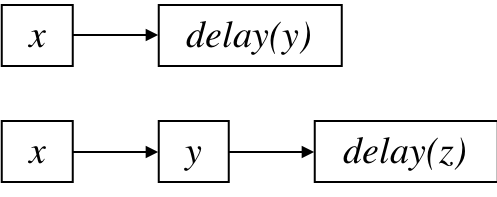
\includegraphics[scale=0.5]{img/stream-cons.eps}
 %\captionsetup{labelformat=empty}
 \caption{The next node pointed is a $\lambda$ expression. It will create a new node when forced evaluation.}
 \label{fig:stream-cons}
%\end{wrapfigure}
\end{figure}

Therefore, when link $x$ and $xs$ together, the value of $xs$ won't be evaluated, but $xs$ itself will be wrapped in a $\lambda$ expression. And evaluation is delayed to future time. With this modification, the generation of natural numbers changes to:

\[
\begin{array}{rcll}
iterate(succ, 0) & = & 0 : iterate(succ, succ(0)) & \text{definition of } iterate\\
                 & = & cons(0, () \mapsto iterate(succ, succ(0))) & \text{lazy link} \\
\end{array}
\]

The computation stops here. It won't go on. The result is a list. The first element is 0, while the next element is a $\lambda$ expression. If we want to obtain the successive element, we have to force the list evaluation.

\[
next(cons(x, e)) = e()
\]

Whey apply $next$ to $cons(0, () \mapsto iterate(succ, succ(0)))$, we obtain:

\[
\begin{array}{cll}
  & next(cons(0, () \mapsto iterate(succ, succ(0)))) & \\
= & iterate(succ, succ(0)) & \text{definition of } next\\
= & iterate(succ, 1) & \text{definition of } succ\\
= & 1 : iterate(succ, succ(1)) & \text{definition of } iterate\\
= & cons(1, () \mapsto iterate(succ, succ(1))) & \text{lazy link}
\end{array}
\]

The computation stops again. By repeatedly applying $next$ to $N$, we generate natural numbers one by one. People call this kind of model {\em stream}, and use it to represent potential infinity. We can easily define a function to fetch the first $m$ natural numbers from this potential infinite stream.

\[
\begin{array}{l}
take\ 0\ \_\ = [] \\
take\ n\ cons(x, e)\ = cons(x, take(n-1, e())) \\
\end{array}
\]

For example, $take\ 8\ N = [0, 1, 2, 3, 4, 5, 6, 7]$. There are examples in the appendix of this chapter about how to define natural numbers with potential infinity in different programming languages.

\begin{Exercise}
\Question{We realized Fibonacci numbers by folding in chapter 1. How to define Fibonacci numbers as potential infinity with $iterate$?}
\Question{Define $iterate$ by folding}
\end{Exercise}

\subsection{Coalgebra and infinite stream$\bigstar$}

To model the stream of potential infinity, we need the coalgebra concept in category theory introduced in chapter 4. Readers are safe skip this section in the following 2 pages, and directly read from the next section \textbf{Explore the actual infinity}. Let us first revisit coalgebra and F-morphism.

\index{coalgebra}
\begin{definition}
\normalfont
Let $\pmb{C}$ be a category, $\pmb{C} \arrowto{\mathbf{F}} \pmb{C}$ is an endo-functor of category $\pmb{C}$. For the object $A$ and morphism $\alpha$ in this category:

\[
  A \arrowto{\alpha} \mathbf{F} A
\]

Form a pair $(A, \alpha)$. It is called F-coalgebra, where $A$ is the carrier object.
\end{definition}

We can treat F-coalgebra as object. When the context is clear, we denote the object as a pair $(A, \alpha)$. The arrows between such objects are defined as the following:

\begin{definition}
\normalfont
F-morphism is the arrow between F-coalgebra objects:

\[
  (A, \alpha) \longrightarrow (B, \beta)
\]

If the arrow $A \arrowto{f} B$ between the carrier objects make the below diagram commutes:

\begin{center}
\begin{tikzpicture}
  \matrix (m) [matrix of math nodes,
               row sep=3em, column sep=3em, minimum width=2em]{
    A & \mathbf{F} A \\
    B & \mathbf{F} B \\};
  \path[-stealth]
    (m-1-1) edge node [above] {$\alpha$} (m-1-2)
    (m-1-1) edge node [left] {$f$} (m-2-1)
    (m-1-2) edge node [right] {$\mathbf{F}(f)$}   (m-2-2)
    (m-2-1) edge node [below] {$\beta$} (m-2-2);
\end{tikzpicture}
\end{center}

Which means $\beta \circ f = \mathbf{F}(f) \circ \alpha$
\end{definition}

F-coalgebra and F-morphism form F-coalgebra category $\pmb{CoAlg}(\mathbf{F})$. For F-algebra, we care about the initial algebra; symmetrically, for F-coalgebra, we care about the {\em final coalgebra}. Where the final coalgebra is the final object in F-coalgebra category, denoted as $(T, \mu)$. For any other algebra $(A, f)$, there exists unique morphism $m$, such that the below diagram commutes:

\begin{center}
\begin{tikzpicture}
  \matrix (m) [matrix of math nodes,
               row sep=3em, column sep=3em, minimum width=2em]{
    \mathbf{F} T & \mathbf{F} A \\
    T & A \\};
  \path[-stealth]
    (m-1-2) edge node [above] {$\mathbf{F}(m)$} (m-1-1)
    (m-2-1) edge node [left] {$\mu$} (m-1-1)
    (m-2-2) edge node [right] {$f$} (m-1-2)
    (m-2-2) edge node [below] {$m$} (m-2-1);
\end{tikzpicture}
\end{center}

From Lambek theorem, the final coalgebra is the fixed point for functor. The morphism $T \arrowto{\mu} \mathbf{F} T$ is an isomorphism, such that $\mathbf{F} T$ is isomorphic to $T$. The final coalgebra can be used to build infinite data structures.

\index{anamorphism}
We use catamorphism to evaluate the initial algebra. Symmetrically, we use anamorphism (prefix ana- means upward) to coevaluate the final coalgebra. For any coalgebra $(A, f)$, the unique arrow to the final coalgebra $(T, \mu)$ can represented with the anamorphism as $\llb f \rlb$. The brackets do not look like bananas any more, but like a pair of lenses in optics. They are known as \textbf{lens brackets}. As shown in below diagram:

\begin{center}
\begin{tikzpicture}
  \matrix (m) [matrix of math nodes,
               row sep=3em, column sep=3em, minimum width=2em]{
    T  & \mathbf{F} T \\
    A  & \mathbf{F} A \\};
  \path[-stealth]
    (m-1-1) edge node [above] {$\mu$} (m-1-2)
    (m-2-1) edge node [left] {$\llb f \rlb$} (m-1-1)
    (m-2-2) edge node [right] {$\mathbf{F}\ \llb f \rlb$}  (m-1-2)
    (m-2-1) edge node [below] {$f$} (m-2-2);
\end{tikzpicture}
\end{center}

\[
  m = \llb f \rlb \text{,if and only if} \mu \circ m = \mathbf{F}(m) \circ f
\]

Let us see how anamorphism builds infinite stream. Anamorphism takes a coalgebra $A \arrowto{f} \mathbf{F} A$ and a carrier object $A$, it generates the fixed point of functor $\mathbf{F}$, which is $\mathbf{Fix}\ \mathbf{F}$. This fixed point is the final coalgebra. It has the form of infinite stream.

\[
\llb f \rlb = \mathbf{Fix} \circ \mathbf{F}\ \llb f \rlb \circ f
\]

We can also define the anamorphism as the function that returns the fixed point:

\[
\begin{array}{l}
(A \to \mathbf{F} A) \arrowto{ana} (A \to \mathbf{Fix}\ \mathbf{F}) \\
ana\ f = Fix \circ fmap\ (ana\ f) \circ f \\
\end{array}
\]

As a concrete example, functor $\mathbf{F}$ is defined as:

\begin{lstlisting}
data StreamF E A = StreamF E A
\end{lstlisting}

Its fixed point is:

\begin{lstlisting}
data Stream E = Stream E (Stream E)
\end{lstlisting}

$\mathbf{StreamF}\ E$ is a normal functor, we intend to give it name of `stream'. The coalgebra of this functor is such a function, it transforms a `seed' $a$ of type $A$ to a pair, containing $a$, and the next seed.

Coalgebra can generates varies of infinite streams. Here are two examples. The first example is Fibonacci numbers. We use $(0, 1)$ as the starting seed. To generate the next seed, we take the second value 1 in the pair as the first value in the new pair, and use $0 + 1$ as the second value in the new pair to form the new seed $(1, 0 + 1)$. Repeat this process, for seed $(m, n)$, we generate the next seed $(n, m + n)$. Written in coalgebra, we have the following definition:

\[
\begin{array}{l}
(Int, Int) \arrowto{fib} \mathbf{StreamF}\ Int\ (Int, Int) \\
fib (m, n) = \mathbf{StreamF}\ m\ (n, m + n)
\end{array}
\]

In this definition, the carrier object $A$ is a pair of integers. With coalgebra, we can feed it into anamorphism to build the infinite stream of Fibonacci numbers. For functor $\mathbf{StreamF}\ E$, the type of the anamorphism is:

\[
(A \to \mathbf{StreamF}\ E\ A) \arrowto{ana} (A \to \mathbf{Stream}\ E)
\]

We can realize it as:

\[
\begin{array}{l}
ana\ f = fix \circ f \\
\text{where: } fix\ (StreamF\ e\ a) = Stream\ e\ (ana\ f\ a)
\end{array}
\]

Apply the anamorphism to coalgebra $fib$ and the start pair $(0, 1)$ gives infinite stream that generates Fibonacci numbers:

\[
ana\ fib\ (0, 1)
\]

We can define a auxiliary function to take the first $n$ elements from the infinite stream:

\begin{lstlisting}
take 0 _ = []
take n (Stream e s) = e : take (n - 1) s
\end{lstlisting}

The next example demonstrates how to generate infinite stream of prime numbers with the sieve of Eratosthenes method. The start seed is `all' the natural numbers with 1 being removed: 2, 3, 4, ... From this seed, we remove all the multiples of 2 to obtain the next seed, which is a infinite list start from 3 as 3, 5, 7, ... Next, we remove all the multiples of 3, and repeated this process. This method is defined as below coalgebra:

\[
\begin{array}{l}
[Int] \arrowto{era} \mathbf{StreamF}\ Int\ [Int] \\
era (p:ns) = \mathbf{StreamF}\ p\ \{ n\ |\ p \nmid n, n \in ns\} \\
\end{array}
\]

Then feed it to anamorphism, we obtain the infinite stream that generate all prime numbers:

\begin{lstlisting}
primes = ana era [2...]
\end{lstlisting}

For list particularly, anamorphism is called unfold. Anamorphism and catamorphism are mutually inverse. We can turn the infinite stream back to list through catamorphism.

\begin{Exercise}
\Question{Use the definition of the fixed point in chapter 4, prove $Stream$ is the fixed point of $StreamF$.}
\Question{Define $unfold$.}
\end{Exercise}

\section{Explore the actual infinity}

Aristotle's influence was profound. For more than two thousand years, mathematicians and philosophers had been thinking about concept of infinity. Most of them accepted the potential infinity. However, there were discordant views about actual infinity. For a long time, people believed the actual infinity was God, or only God mastered actual infinity. Many attempts to reasoning the actual infinity led to confusion and contradict result. For example, let all the natural numbers be actual infinity. Because from the beginning, natural numbers are separated by even numbers and odd numbers. They alternate in turns. It's natural to think that all even numbers are half of all natural numbers. However, doubling every natural number gives an even number; and dividing every even number by 2 gives a natural number vise versa. Then there is one to one correspondence between all the natural numbers and even numbers. Are these two actual infinities same? If not, which one has more? natural numbers or even numbers?

\index{Galileo's paradox}
Father of the modern science, Galileo Galilei made a similar paradox in his final scientific work {\em Two New Sciences} in 1636. First, some numbers are squares, while others are not; therefore, all the numbers, including both squares and non-squares, must be more numerous than just the squares. And yet, for every number there is exactly one square. Forms the sequence 1, 4, 9, 16, 25, ... hence, there cannot be more of one than of the other. This paradox is known as Galileo's paradox.

Not only for numbers, people found similar paradox in Geometry. As shown in figure \ref{fig:circles-paradox}, For two circles with the same center, every radius connects two points in each circle respectively, hence, there is one to one correspondence between the points in the bigger circle and the smaller circle. It indicates there are same many points in each circle. However, our common sense tells there must be more points in the bigger one.

\begin{figure}[htbp]
%\begin{wrapfigure}{L}{0.4\textwidth}
 \centering
 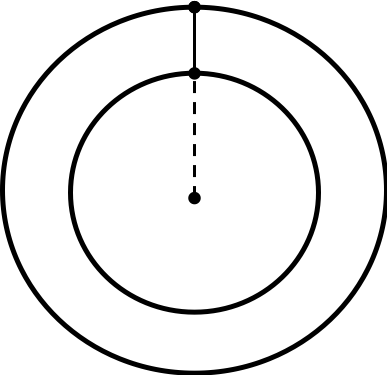
\includegraphics[scale=0.5]{img/circles-paradox.eps}
 %\captionsetup{labelformat=empty}
 \caption{Every point in the big circle is corresponding to a point in the small circle.}
 \label{fig:circles-paradox}
%\end{wrapfigure}
\end{figure}

Because of these paradoxes, people accepted Aristotle's approach to avoid using actual infinity. Galileo concluded that the ideas of less, equal, and greater couldn't apply to infinite sets like natural numbers. People rejected terms of actual infinity, like ``all the natural numbers''.

%\begin{figure}[htbp]
\begin{wrapfigure}{R}{0.4\textwidth}
 \centering
 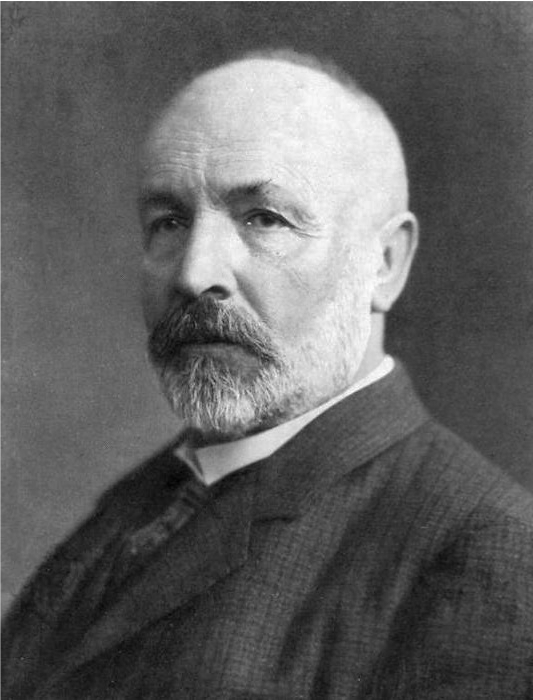
\includegraphics[scale=0.5]{img/Cantor.eps}
 \captionsetup{labelformat=empty}
 \caption{Georg Cantor, 1845-1918}
 \label{fig:Cantor}
\end{wrapfigure}
%\end{figure}

About two hundred years after Galileo, German mathematician Cantor led people broke into the Kingdom of infinity. From these paradoxes, Cantor thought the key problem lay in our common sense assumption, that the whole must be larger than the part. Is it necessarily right? The development of modern science taught us our common view to things could be incomplete or wrong. The theory of relativity challenges our understanding to space and time -- the space we are living in is not necessarily the Euclidean space; Quantum mechanics challenges our common sense that the world is causal -- randomness rules the quantum world. When think out of the box, it will open up a new world we've never seen, resulting in fundamental development. This was exactly what Cantor did. If we accept the counter-intuitive result, that `the part can equal to the whole', then the door to the infinity is open. He established the importance of one-to-one correspondence between the members of two sets, and defined (actual) infinite sets.

To compare two sets, Cantor defined if there is one to one correspondence between them, that every element in set $M$ has the unique corresponding element in set $N$, then the two sets are equinumerous. That is of the same size or having the same number of elements\footnote{Remind the `isomorphic' concept we introduced in chapter 3.}. For finite sets, it is true obviously, when extends to infinite sets, it means there are same infinite many even numbers as the natural numbers! there are same infinite many square numbers as natural numbers, the points in smaller circle and the bigger circle of the same center are equinumerous... Cantor's friend, Richard Dedekind even gave such a definition\footnote{known as Dedekind infinite set nowadays.} of infinite set in 1888: if some proper subset of a set is equinumerous to this set, then it is a infinite set.

% Cardinality vs. cardinal number

\subsection{Paradise of infinite kingdom}

Let us have a glance view of the garden in infinite kingdom. David Hilbert told an interesting story in a lecture in 1924 (published in 2013) to help people understanding Cantor's infinite sets. It was popularized through George Gamow's 1947 book {\em One Two Three... Infinity}.

In this story, there is a Grand hotel with infinite many rooms. It is fully occupied during the hot season. In the evening, a tired driver has passed many ``No vacany'' hotels before reaching to this one. He goes to see if there might nonetheless be a room for him. The clerk, Hilbert said: ``No problem, we can make a room for you.'' He asked the guest in room 1 to move to room 2, then moved the guest in room 2 to room 3, and moved the guest in room 3 to room 4, ... He moved every one from current room to the next room. That freed up the first room for this new guest.

The story goes on. On the second day, there comes a tour group of infinite many guests. Hilbert said: ``No problem, we can make rooms for every one.'' He asked the new guest who was in room 1 last night to move to room 2, then moved the guest in room 2 to room 4, and moved the guest in room 3 to room 6, ... He moved every one in room $i$ to room $2i$. Since the hotel has infinite many rooms, after moving, room 2, 4, 6, ... these even number rooms are occupied with the guests accommodated yesterday, while the room 1, 3, 5, ... these odd number rooms are free up. There are infinite many odd numbers rooms that can accommodate every member in the tour group.

The story does not end. On the third day, there comes infinite many tour groups of infinite many guests each. Can the magic Hilbert's hotel accommodate them all? Before see the answer, let us first revisit the story on the first two days.

\begin{figure}[htbp]
%\begin{wrapfigure}{R}{0.4\textwidth}
 \centering
 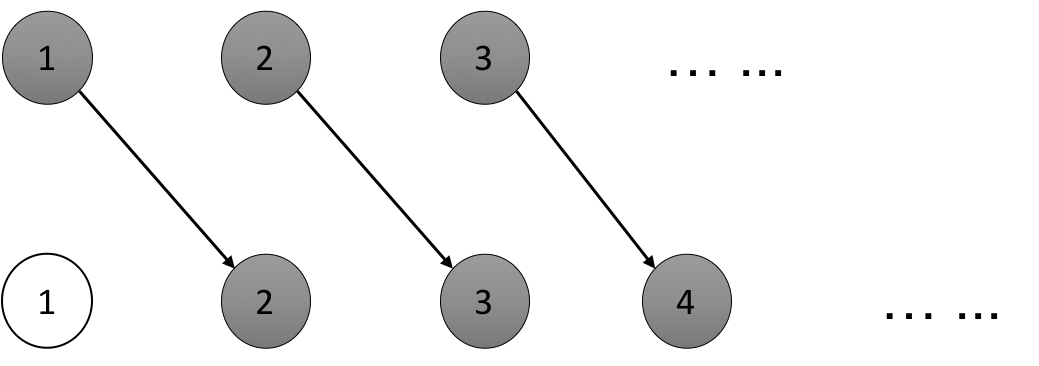
\includegraphics[scale=0.4]{img/Hilbert-hotel-1.eps}
 %\captionsetup{labelformat=empty}
 \caption{First day of Hilbert's Grand hotel}
 \label{fig:Hilbert-hotel-1}
%\end{wrapfigure}
\end{figure}

As shown in figure \ref{fig:Hilbert-hotel-1}, on the first day, we move every guest to the next room to free up room 1. Essentially, we establish a 1-to-1 correspondence for shadowed circles between the two rows as $n \leftrightarrow n+1$. It reveals a counterintuitive fact that infinity plus one is infinity again. Hilbert's grand hotel can accommodate not only this one more guest, but also finite many $k$ new guests by repeating this arrangement $k$ times. It means:

\bean
\infty + 1 = \infty \\
\infty + k = \infty \\
\eean

\begin{figure}[htbp]
%\begin{wrapfigure}{R}{0.4\textwidth}
 \centering
 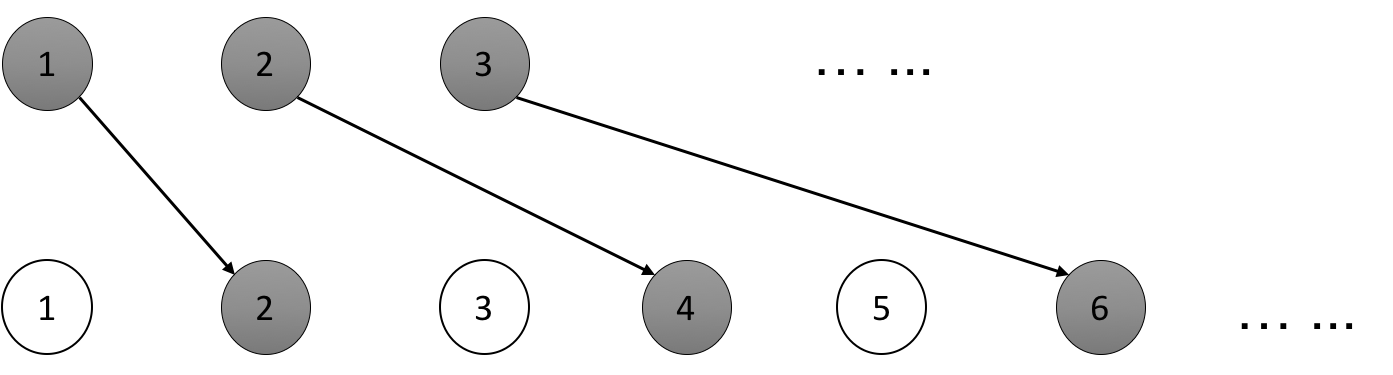
\includegraphics[scale=0.4]{img/Hilbert-hotel-2.eps}
 %\captionsetup{labelformat=empty}
 \caption{Second day of Hilbert's Grand hotel}
 \label{fig:Hilbert-hotel-2}
%\end{wrapfigure}
\end{figure}

The solution for the second day is shown in figure \ref{fig:Hilbert-hotel-2}. We essentially establish a 1-to-1 correspondence between natural numbers and even numbers, hence free up infinite many odd number rooms. Then we establish another 1-to-1 correspondence between these empty rooms and the infinite many guests in the tour group, which is exactly the 1-to-1 correspondence between odd numbers and natural numbers. The second day story tells us, infinity plus infinity is infinity again.

\[
\infty + \infty = \infty
\]

It's natural to ask, although the symbols are same, does the infinity on the left hand equal to the infinity on the right hand? Can we compare between infinities for size? We'll see later, it was exactly this question, led Cantor to study infinity in depth. In Hilbert's Grand hotel story, we can establish 1-to-1 correspondence between all these infinities, hence they are all equinumerous. Such infinity that has 1-to-1 correspondence with natural numbers are called `countable infinity'.

To solve the problem on the third day of Hilbert's Grand hotel, we need think about how to establish the 1-to-1 correspondence between the infinite many tour groups of infinity many guests and the infinity many rooms. One may come to the idea to arrange the guests in the first tour group to room 1, 2, 3, ... then arrange the guests in the second group to room $\infty + 1$, $\infty + 2$, ... However, this method does not work. We don't know which one are more numerous, the rooms or the guests before the arrangement. Consider how this process executes. The first guest in the second group will never know when the first group finishes accommodating, this guest has no way to determine which room should move to. Compare with the first day story, the new guest could immediately move to room 1 when the original guest moved to room 2, although the whole infinity accommodating process is endless. Same situation happened on the second day. When the original guest in room 1 moved to room 2, the first guest in the tour group could move to the freed up room 1 immediately. Next the original guest in room 2 moved to room 4, and the guest in room 3 moved to room 6, at this time, the second guest in the tour group could move to room 3...

\begin{figure}[htbp]
\centering
\begin{tikzpicture}
  \draw[step=1, very thin, gray] (0, 0) grid (5, 5);
  \draw[->] (-0.25, 0) -- (6, 0) coordinate (x axis);
  \draw[->] (0, -0.25) -- (0, 6) coordinate (y axis);
  \foreach \x in {0, 1, 2, 3, 4, 5}
    \path (\x, -0.25) node[left] {\x};
  \foreach \y in {1, 2, 3, 4, 5}
    \path (-0.25, \y) node[below] {\y};
  \foreach \i / \x / \y in {0/0/0, 1/1/0, 2/0/1, 3/0/2, 4/1/1, 5/2/0, 6/3/0, 7/2/1, 8/1/2, 9/0/3, 10/0/4}{
    \path (\x, \y) coordinate (N\i);
    \fill (N\i) circle (1pt) node[above right=3pt of N\i] {\i};
  }
  \foreach \i in {0,...,9} {
    \pgfmathsetmacro{\j}{\i+1}
    \draw[-latex, thick] (N\i) to (N\j);
  }
\end{tikzpicture}
\caption{One solution to number the infinity of infinity}
\label{fig:NNtoN}
\end{figure}

Figure \ref{fig:NNtoN} gives a numbering solution. For convenient purpose, we label the first guest 0, the second guest 1, the third guest 2, ... We label the guests already lived in the hotel as group 0, the first tour group 1, the second group 2, ... In this figure, every guest corresponds to a grid point. We also count the hotel rooms from 0.

Now we arrange rooms in this order: assign the guest 0 in group 0 to room 0, the guest 1 in group 0 to room 1, the guest 0 in group 1 to room 2, the guest 0 in group 2 to room 3, the guest 1 in group 1 to room 4, ... Along the zig-zag path, we can assign room one by one, without missing any guests. Hence we establish a 1-to-1 correspondence between every guest in these infinite many groups and the infinity many rooms. Hilbert's Grand hotel surprisingly holds `two-dimensional' infinity\footnote{The traditional solution uses the Euclid's theorem, that there are infinite many prime numbers. Empty the odd numbered rooms by sending the guest in room $i$ to room $2^{i}$, then put the first group's guests in rooms $3^{n}$, the second group's guests in rooms $5^{n}$, ... put the $k$-th group's guests in rooms $p^n$, where $p$ is the $k$-th prime number. This solution leaves certain rooms empty, specifically, all odd numbers that are not prime powers, such as 15 or 847, will no longer be occupied.}.

\begin{Exercise}
\Question{We establish the 1-to-1 correspondence between the rooms and guests with the numbering scheme shown in \ref{fig:NNtoN}. For guest $i$ in group $j$, which room number should be assigned? Which guest in which group will live in room $k$?}
\Question{For Hilbert's Grand hotel, there are multiple solutions for the problem on the third day. Figure \ref{fig:PWW-NNtoN} is the cover page of the book {\em Proof without word}. Can you give a numbering scheme based on this figure?
\begin{figure}[htbp]
 \centering
 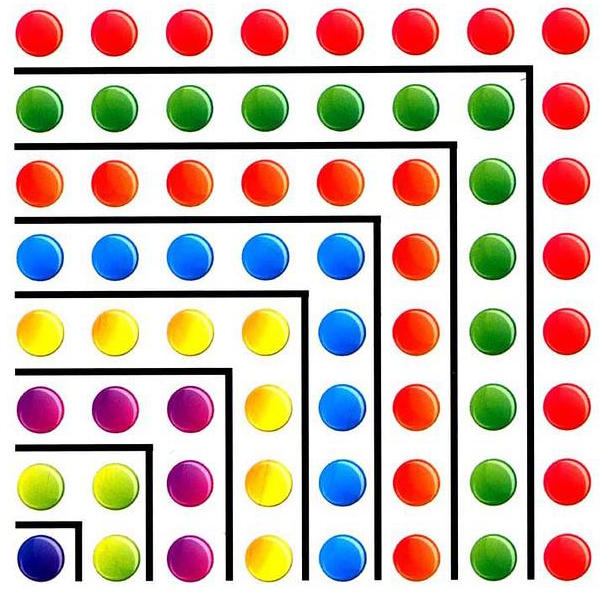
\includegraphics[scale=0.2]{img/PWW.eps}
 \caption{From cover page of {\em Proof without word}}
 \label{fig:PWW-NNtoN}
\end{figure}
}
\end{Exercise}

\subsection{One-to-one correspondence and infinite set}

From Hilbert's Grand hotel story, we see the importance of the 1-to-1 correspondence when study infinity. If there exists 1-to-1 correspondence between two sets, then they have the same cardinality. We can further use 1-to-1 correspondence to classify sets. As explained in chapter 3, for two sets $A$ and $B$, we establish a map $A \arrowto{f} B$, such that every element $x$ in $A$ is corresponding to an element $y$ in $B$ through $x \mapsto y = f(x)$. For sets, we call $f$ function. $y$ is the image of $x$, and $x$ is preimage. If there is exactly one preimage, such map is called {\em injective function}; if every element $y$ in $B$ has a preimage, then the map is called {\em surjective} or onto. If a map is both injective and surjective, it is called bijective or one-to-one correspondence. Figure \ref{fig:bijection} illustrates a bijection between two sets.

\begin{figure}[htbp]
%\begin{wrapfigure}{R}{0.4\textwidth}
 \centering
 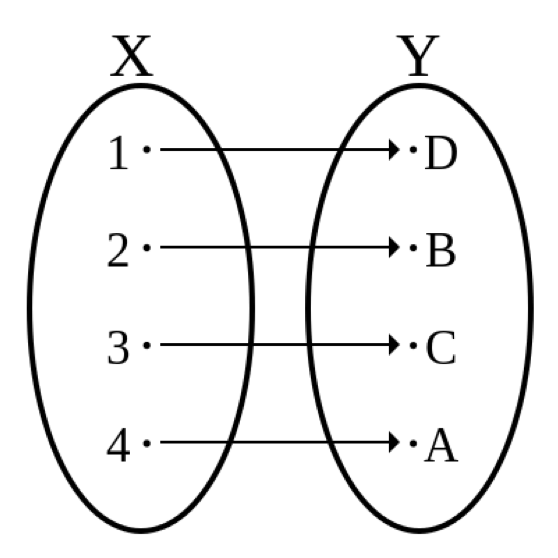
\includegraphics[scale=0.4]{img/bijection.eps}
 %\captionsetup{labelformat=empty}
 \caption{1-to-1 correspondence between two sets.}
 \label{fig:bijection}
%\end{wrapfigure}
\end{figure}

Hilbert's Grand hotel gives surprisingly counterintuitive properties of infinity. The set of natural numbers is equinumerous with its proper subsets like even and odd numbers. And the one dimensional natural number $n$ and two dimensional pair $(m, n)$ are also equinumerous. Starting from natural numbers, Cantor expanded a series of infinite sets through 1-to-1 correspondence. for example:

\begin{enumerate}
\item \textbf{Integers}. We can establish the following 1-to-1 correspondence:

\begin{tabular}{ccccccccc}
0 & 1 & -1 & 2 & -2 & ... & $n$ & $-n$ & ... \\
$\updownarrow$ & $\updownarrow$ & $\updownarrow$ & $\updownarrow$ & $\updownarrow$ & & $\updownarrow$ & $\updownarrow$ & \\
0 & 1 &  2 & 3 &  4 & ... & $2n - 1$ & $2n$ & ... \\
\end{tabular}

Hence to expand natural numbers to integers. From another view point, we essentially correspond odd numbers to positive integers, and correspond even numbers to negative integers and zero. It tells that the integers and natural numbers are equinumerous.

\item \textbf{Rationals}. A rational number can be expressed as the quotient or fraction $p/q$ of two integers, a numerator $p$ and a non-zero denominator $q$. On the third day of Hilbert's Grand hotel story, we established 1-to-1 correspondence between a pair $(p, q)$ and a natural number. We can adjust it a bit for rational number $p/q$. Put negative numbers aside for now, we skip whenever the second number $q$ is zero, or $p/q$ is irreducible fraction (no common divisor). Then we re-use the method for integers, to cover the negative rational numbers as well. In this way, we construct rational numbers from natural numbers. Below table illustrates how the first several natural numbers correspond to rational numbers:

\begin{tabular}{cccccccccc}
0 & 1 & 2 & 3 & 4 & 5 & 6 & 7 & 8 & ... \\
$\updownarrow$ & $\updownarrow$ & $\updownarrow$ & $\updownarrow$ & $\updownarrow$ & $\updownarrow$ & $\updownarrow$ & $\updownarrow$ & $\updownarrow$ & \\
0 & 1 & $\dfrac{1}{2}$ & $-\dfrac{1}{2}$ & -1 & -2 & $-\dfrac{2}{3}$ & $-\dfrac{1}{3}$ & $\dfrac{1}{3}$ & ... \\
\end{tabular}

It tells us natural numbers and rational numbers are equinumerous.

\index{algebraic numbers}
\item \textbf{Algebraic numbers}. An algebraic number is a root of a non-zero polynomial in one variable with rational coefficients. Equivalently, by clearing denominators, we can loose the coefficients to integers. For example, $\sqrt{2}$ and $1 \pm \sqrt{3}i$ are algebraic numbers, while $\pi$ and $e$ are not.

Given an algebraic equation

\[
a_0 x^n + a_1 x^{n-1} + ... + a_n = 0
\]

Where $a_0, a_1, ... a_n$ are integers, and $a_0 \neq 0$. All its rots are algebraic numbers. Define a positive integer:

\[
h = n + |a_0| + |a_1| + ... + |a_n|
\]

Which is the sum of the degree and coefficients of the equation. We name it as the height $h$ of the equation. For any algebraic equation, $h$ is a unique natural number. On the other hand, given a height $h$, there could be multiple equations. For example, the height of equations $x - 3 = 0$, $x^3 + 1 = 0$, $x^3 - 1 = 0$, $x^2 + x + 1 = 0$, $x^2 - x + 1 = 0$ are all 4. However, there are finite many equations for a every $h$. Therefore, we can enumerate all algebraic equations: first list all equations of height $h=1$, then list the equations of height $h=2$, ... and repeated this process. The equations of the same heights can be list in arbitrary order. According to the fundamental theorem of algebra proved by Gauss, the number of roots equals to the equation degree $n$. Taking the multiplicity into consideration, the number of different roots is not greater than $n$. Hence there are finite many roots for equation of height $h$. Now we can enumerate all algebraic numbers.

First, we enumerate all roots for equations of height $h=1$ (only one such equation $x = 0$), which is 0; then enumerate all roots for equations of height 2. Because different equations may have some same root, we need skip any root if it was enumerated before. In this way, we establish the 1-to-1 correspondence between algebraic numbers and natural numbers. Hence they are equinumerous. In other words, we can extend to all algebraic numbers from natural numbers.
\end{enumerate}

We'll meet a problem next. Can we extend natural numbers to real numbers? not only for normal irrationals, but also cover transcendental numbers like $\pi$ and $e$? Cantor and Dedekind made great breakthrough when study this problem.

\subsubsection{Cantor and Dedekind}

%\begin{figure}[htbp]
\begin{wrapfigure}{R}{0.4\textwidth}
 \centering
 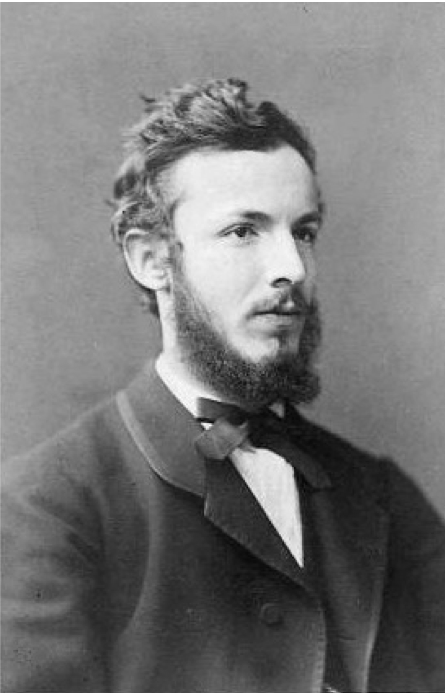
\includegraphics[scale=0.5]{img/Cantor-1870.eps}
 \captionsetup{labelformat=empty}
 \caption{Cantor, around 1870}
 \label{fig:Cantor-1870}
\end{wrapfigure}
%\end{figure}

\index{Cantor}
Georg Cantor was a German mathematician, He created set theory, which has became a fundamental theory in mathematics. Cantor was born in 1845 in the western merchant colony of Saint Petersburg, Russia, and brought up in the city until he was eleven. His father was a successful merchant, and member of the Saint Petersburg stock exchange; his mother came from a family well-known of music. When his father became ill, the family moved to Germany Frankfurt in 1856. Cantor demonstrated exceptional skill in mathematics in school. But his father wanted Cantor to became ``a shining star in the engineering firmament.'' However, at the age of 17, Cantor had sought his father's permission to study mathematics at university and he was overjoyed when eventually his father consented\cite{HanXueTao16}.

He entered the Polytechnic of Zürich in 1862, then moved to the University of Berlin in 1863. He attended lectures by Leopold Kronecker, Karl Weierstrass and Ernst Kummer. He spent the summer of 1866 at the University of Göttingen. Cantor was a good student, and he received his doctorate degree in 1867 with the dissertation on number theory. Cantor later took up a position at the University of Halle, where he spent his entire career.

At that time, many mathematicians were trying to rebuild the rigorous logical foundation of analysis led by Weierstrass. Cantor also influenced by this movement. He soon realized the importance to study real numbers as the basis of calculus, which became the beginning of set theory research.

In 1872, he met and began a friendship with the young mathematician Richard Dedekind while on holiday in Switzerland. Even in Cantor's honeymoon in Harz mountains, Cantor spent much time in mathematical discussions with Dedekind. They started a long time correspondence between each other.

In 1874, Cantor published his first revolutionary paper about set theory at the age of 29. It marked as the beginning of set theory as a branch of mathematics. With the extraordinary ingenuity, Cantor established set theory in the following ten years almost alone, leading the revolution of infinity in mathematics. However, he was not well recognized during his most creative period. He desired, but was not able to obtain a professor chair at the University of Berlin. He spent his career at the University of Halle, which was a infamous university with a meager salary. Cantor's theory was originally regarded as so counter-intuitive – even shocking. People found paradoxes hidden in infinity sets (we'll introduce Russell's paradox in next chapter). Cantor's work encountered resistance from mathematical contemporaries. Among them, some were famous mathematicians, including his teacher, the leading mathematician in Berlin, Leopold Kronecker. He had a famous saying: ``God made the integers, all else is the work of man.'' He objected to Cantor's theory about infinity and transcendental numbers, said it was not mathematics but mysticism. Mathematics was headed for the madhouse under Cantor's leadership. Henri Poincaré, the famous French mathematician, known as ``The Last Universalist'', referred to Cantor's work as a ``disease'' from which mathematics would eventually be cured. Poincaré said, ``There is no actual infinite; the Cantorians have forgotten this, and that is why they have fallen into contradiction.''. Later Hermann Weyl, the great German mathematician criticized Cantor's hierarchy of infinities as ``fog on fog.'' Hermann Schwartz was originally a friend of Cantor, but he stopped the correspondence with Cantor as opposition to Cantor's ideas continued to grow. Mathematicians split to schools of empiricism, intuitionism, and constructivism in different ways, and fell into the controversy about the foundations of mathematics against Cantor.

The tragedy was not the set theory, but Cantor went to the madhouse. Cantor suffered his first known bout of depression in May 1884. During the rest of his life, the depression recurred several times with different intensity, driving him from the community into the mental hospital refuge. In 1904 he was agitated by a paper presented by Julius König at the Third International Congress of Mathematicians. The paper was read in front of his daughters and colleagues. Cantor was shaken, and sent to hospital again. Cantor retired in 1913, living in poverty. In June 1917, he entered the sanatorium for the last time and continually wrote to his wife asking to be allowed to go home. Cantor died on January 6, 1918, in the sanatorium where he had spent the last year of his life.

Cantor's set theory was publicly acknowledged and praised at the first International Congress of Mathematicians, held in Zurich in 1897. Adolf Hurwitz (1859 - 1919) openly expressed his great admiration of Cantor and proclaimed him as one by whom the theory of functions has been enriched. Jacques Hadamard expressed his opinion that the notions of the theory of sets were known and indispensable instruments. Over time, people gradually realized the importance of set theory. David Hilbert praised Cantor's work as ``the finest product of mathematical genius and one of the supreme achievements of purely intellectual human activity.'' The Continuum hypothesis, introduced by Cantor, was presented by Hilbert as the first of his twenty-three open problems in his address at the 1900 International Congress of Mathematicians in Paris. When Brouwer, the founder of intuitionism criticizing the paradoxes in set theory, Hilbert defended it by declaring, ``No one shall expel us from the paradise that Cantor has created.''

%\begin{figure}[htbp]
\begin{wrapfigure}{L}{0.4\textwidth}
 \centering
 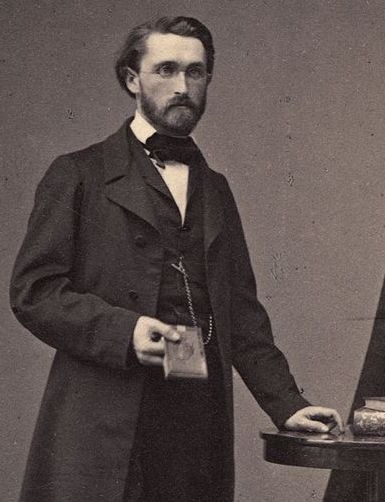
\includegraphics[scale=4]{img/Dedekind.eps}
 \captionsetup{labelformat=empty}
 \caption{Richard Dedekind, 1831-1916}
 \label{fig:Dedekind}
\end{wrapfigure}
%\end{figure}

\index{Dedekind}
Richard Dedekind was a German mathematician, educationist. He was born on October 6, 1831 in Brunswick Germany, where is the hometown of Gauss. His father was a professor, his mother was a daughter of a professor at the same university in Brunswick. When Dedekind was in school, mathematics was not his main interest. He studied science, in particular physics and chemistry. However, they became less than satisfactory to Dedekind with what he considered an imprecise logical structure and his attention turned towards mathematics. He entered the University of Göttingen in the spring of 1850 with a solid grounding in mathematics. He learned number theory from M A Stern, and physics from Wilhelm Weber. Gauss was still teaching, although mostly at an elementary level, and Dedekind became his last student. Dedekind did his doctoral work in four semesters under Gauss's supervision and submitted a thesis on the theory of Eulerian integrals. He received his doctorate from Göttingen in 1852.

After that, Dedekind went to Berlin for two years of study, where he and Bernhard Riemann were contemporaries; they were both awarded the habilitation degrees in 1854. Dedekind was then qualified as a university teacher and he began teaching at Göttingen giving courses on probability and geometry. He studied for a while with Dirichlet, and they became good friends. About this time, Dedekind studied the work of Galois and he was the first to lecture on Galois theory. He also became one of the first people to understand the importance of the notion of groups for algebra and arithmetic.

Dedekind was humble. Many of his achievements were unknown to the people at the time. For example, after Dirichlet's death, Dedekind wrote and published the famous book {\em Lectures on Number Theory} based on his notes from Dirichlet's lectures. Dedekind was so modest that he published the book under Dirichlet’s name, even after adding many additional results of his own in later editions. Unfortunately, Dedekind’s modesty hurt his career; he failed to get tenure at Göttingen and ended up on the faculty of a minor technical university(\cite{Stepanov} pp.140). -- Institute of Technology Brunswick in his hometown.

Dedekind remained in Brunswick for the rest of his life, retiring on April 1, 1894. He lived his life as a professor in Brunswick.
``In close association with his brother and sister, ignoring all possibilities of change or attainment of a higher sphere of activity. The small, familiar world in which he lived completely satisfied his demands: ... there he found sufficient leisure and freedom for scientific work in basic mathematical research. He did not feel pressed to have a more marked effect in the outside world: such confirmation of himself was unnecessary.''

Dedekind made a number of highly significant contributions to mathematics and his work would change the style of mathematics into what is familiar to us today. While teaching calculus for the first time at Brunswick, Dedekind developed the notion now known as a Dedekind cut, now a standard definition of the real numbers. As well as his analysis of the nature of number, his work on mathematical induction, including the definition of finite and infinite sets, and his work in number theory, particularly in algebraic number fields, is of major importance. He introduced the notion of an ideal which is fundamental to ring theory (later introduced and extended by Hilbert and Emmy Noether). He also proposed an axiomatic foundation for the natural numbers, whose primitive notions were the number one and the successor function. The next year, Giuseppe Peano, citing Dedekind, formulated an equivalent but simpler set of axioms.

Dedekind died on February 12, 1916. About his death, there was an interesting story. One day, Dedekind discovered in a ``Biography of Mathematicians'', that wrote: Dedekind died on September 4, 1897. To correct this error, he wrote a letter to the editor of the biography: ``According to my diary, I was very healthy on this day and talking with my lunch guest, dear friend Cantor, some interesting things, very enjoyable. "\cite{HanXueTao16}

Even today, there are still different views regarding to Cantor and Dedekind's work. Dieudonné still considered Dedekind's work caused unnecessary confusions in the 1980s. Not to mention the fierce divisions and debates at the beginning of the 20th Century. Most biographies and comments we see today are often too critical to Kronecker, Brouwer, and the mathematical philosophy of intuitionism they represented. They sympathize with Cantor, and enthusiastically praise the revolution of infinite sets and transcendental numbers. We recommend the rational readers have your own thoughts, but not completely influenced by one-sided view or the other. Kronecker had a strong belief in mathematical philosophy. He emphasized that mathematics should deal only with finite numbers and with a finite number of operations. He was the first to doubt the significance of non-constructive existence proofs. We should not think that Kronecker's views of mathematics were totally eccentric. Although it was true that most mathematicians of his day would not agree with those views, and indeed most mathematicians today would not agree with them, they were not put aside. Kronecker's ideas were further developed by Poincaré and Brouwer, who placed particular emphasis upon intuition. Intuitionism stresses that mathematics has priority over logic, the objects of mathematics are constructed and operated upon in the mind by the mathematician, and it is impossible to define the properties of mathematical objects simply by establishing a number of axioms. Poincaré in his famous book {\em  Science and Hypothesis} stated that convention plays an important role in physics. His view came to be known as ``conventionalism''. He also believed that the geometry of physical space is conventional. His idea inspired Einstein when developed his theory of relativity.

\subsubsection{Fibonacci numbers and Hamming numbers}

Some programming environments support lazy evaluation by default. With them, we can perform complex computation directly on infinite streams. Below is a definition of natural numbers.

\[
N = 0 : map(succ, N)
\]

In this definition, $N$ is a infinite set for natural numbers. The first number is zero, from the second one, every number is the successor of the previous natural number, as described in the following table:

\begin{tabular}{|r|r|l|l|l|l|}
\hline
                 & $N$: & 0 & 1 & 2 & ... \\
\hline
                 & $map(succ, N)$: & $succ(0)$ & $succ(1)$ & $succ(2)$ & ... \\
\hline
$0 : map(succ, N)$: & 0 & 1 & 2 & 3 & ... \\
\hline
\end{tabular}

Based on this idea, below example code firstly define the infinite set of natural numbers, then take the first 10 numbers:

\lstset{frame=single}
\begin{lstlisting}
nat = 0 : map (+1) nat

take 10 nat
[0,1,2,3,4,5,6,7,8,9]
\end{lstlisting}

Similarly, we can define Fibonacci numbers as an infinite set. Let $F$ be the set of all Fibonacci numbers. The first element is 0, the second is 1, every Fibonacci number after them are the sum of the previous two. We can make a table with the same method as we do for natural numbers:

\begin{tabular}{|r|r|l|l|l|l|l|l|l|l|}
\hline
  & $F$:  & 0 & 1 & 1 & 2 & 3 & 5 & 8 & ... \\
\hline
  & $F'$: & 1 & 1 & 2 & 3 & 5 & 8 & 13 & ... \\
\hline
0 & 1     & 1 & 2 & 3 & 5 & 8 & 13 & 21 & ... \\
\hline
\end{tabular}

Where the first row lists all Fibonacci numbers; the second row lists removes the first one, and lists the rest. We can also consider it is the result by shifting the first row to left by one cell; in the third row, every cell is the sum of the above two numbers in the same column. It also lists all Fibonacci numbers except for the first two: 0 and 1. We can prepend them to the left of the third row to obtain the definition of infinite Fibonacci numbers:

\[
F = \{0, 1\} \cup \{ x + y | x \in F, y \in F'\}
\]

Here is the corresponding example code:
\begin{lstlisting}
fib = 0 : 1 : zipWith (+) fib (tail fib)
\end{lstlisting}

\index{regular numbers} \index{Hamming numbers}
Here is another example, in mathematics, regular numbers are defined as those numbers whose only prime divisors are 2, 3, and 5. In computer science, regular numbers are often called Hamming numbers, after Richard Hamming (American mathematician, ACM Turning award receiver, 1915-1998), who proposed the problem of finding computer algorithms for generating these numbers in ascending order. Here are the first several Hamming numbers.

\[
1, 2, 3, 4, 5, 6, 8, 9, 10, 12, 15, 16, 18, 20, 24, 25, 27, 30, 32, 36, 40, 45, 48, 50, 54, 60, ...
\]

It's not trivial to write a program to generate Hamming numbers. While there exits an intuitive and efficient method by using infinite stream. Let $H$ be the infinite set of Hamming numbers. The first Hamming number is 1. For every number $x$ in $H$, $2x$ is still a Hamming number. It means $H_2 = \{ 2x | x \in H \}$. It is also true for factor 3 and 5, hence we have $H_3 = \{ 3x | x \in H \}$ and $H_5 = \{ 5x | x \in H \}$ respectively. If we merge these three sets, $H_1, H_3$, and $H_5$ together, remove those duplicated numbers, and prepend 1, then we obtain the set of Hamming numbers again.

\[
\begin{array}{rcl}
H & = & \{ 1 \} \cup H_2 \cup H_3 \cup H_5 \\
  & = & \{ 1 \} \cup \{ 2x | x \in H \} \cup \{ 3x | x \in H \} \cup \{ 5x | x \in H \} \\
\end{array}
\]

In programming, $\cup$ means merge two series $X = \{x_1, x_2, ...\}$ and $Y = \{y_1, y_2, ...\}$ in order, and drop the duplicated elements.

\[
X \cup Y =
\begin{cases}
x_1 < y_1 : & \{x_1, X' \cup Y \} \\
x_1 = y_1 : & \{x_1, X' \cup Y' \} \\
x_1 > y_1 : & \{y_1, X \cup Y' \} \\
\end{cases}
\]

Here is an example code that summarizes above definition, and returns the 1,000,000th Hamming number.

\begin{lstlisting}
ham = 1 : map (*2) ham # map (*3) ham \# map (*5) ham
  where xxs@(x:xs) # yys@(y:ys)
    | x==y = x : xs # ys
    | x<y  = x : xs # yys
    | x>y  = y : xxs # ys

ham !! 1000000
519312780448388736089589843750000000000000000000000000
000000000000000000000000000000
\end{lstlisting}

\lstset{frame=none}

\subsection{Countable and uncountable infinite}
\index{countable set}
From natural numbers, we've seen how to construct integers, rationals, and the algebraic numbers (including part of irrational numbers like radicals). We are able to establish 1-to-1 correspondence between all of them and natural numbers, hence they are all equinumerous. A set is called {\em countable} infinite set if it has the same cardinality as natural numbers. Are all infinite set countable? Are there any larger infinities? On November 29, 1873, Cantor wrote to his friend Dedekind a letter(\cite{Calvin-Clawson-1994}, pp. 198).

\begin{quotation}
May I ask you a question, which has a certain theoretical interest for me. but which I can't answer; may be you can answer it and would be so kind as to write to me about it. It goes as follows: take the set of all natural numbers $n$ and denote it $N$. Further, consider, say, the set of all positive real numbers $x$ and denote it $R$. Then the question is simply this: can $N$ be paired with $R$ in such a way that to every individual of one set corresponds to one and only one individual of the other? At first glance, one says to oneself, ``No, this is impossible, for $N$ consists of discrete parts and $R$ is a continuum.'' But nothing is proved by this objection. And much as I too feel that $N$ and $R$ do not permit such a pairing, I still cannot find the reason. And it is this reason that bothers me; maybe it is very simple.
\end{quotation}

\index{diagonal method}

One week after on December 7, Cantor wrote again to Dedekind.

\begin{quotation}
Recently I had time to follow up a little more fully the conjecture which I mentioned to you; only today I believe I have finished the matter. Should I have been deceived, I would not find a more lenient judge than you. I thus take the liberty of submitting to your judgement what I have written, in all the incompleteness of a first draft.
\end{quotation}

Cantor proved it impossible to establish 1-to-1 correspondence between natural numbers and real numbers, hence real numbers are uncountable. December 7, 1973 was the day that set theory born. Cantor had given two proofs. The second one is the popular Cantor's {\em diagonal argument}.

Cantor used the proof by contradiction method. Suppose the real numbers in open interval $(0, 1)$ are countable. There exits 1-to-1 correspondence to natural numbers. We can list all real numbers in this interval as a sequence $a_0, a_1, a_2, ..., a_n, ...$ in decimals. For any irrational number, its decimal format is endless non-repeating; For rational number, its decimal format can be infinitely repeating finite sequence of digits, for example $\dfrac{1}{3} = 0.333...$; for decimals with finite digits, we can append infinite many zeros, for example $\dfrac{1}{2} = 0.5000...$ All the real numbers in interval $(0, 1)$ can be list as below:

\[
\begin{array}{l}
a_0 = 0.a_{00}a_{01}a_{02}a_{03}...\\
a_1 = 0.a_{10}a_{11}a_{12}a_{13}...\\
a_2 = 0.a_{20}a_{21}a_{22}a_{23}...\\
a_3 = 0.a_{30}a_{31}a_{32}a_{33}...\\
... \\
a_n = 0.a_{n0}a_{n1}a_{n2}a_{n3}...\\
... \\
\end{array}
\]

Here is an important note: $a_0, a_1, a_2, ...$ are not necessarily ordered from small to big. Next we construct a number $b = 0.b_0b_1b_2b_3...b_n...$, where the $n$-th digit $b_n \neq a_{nn}$. To achieve this, we can simply make a rule, if $a_{nn} \neq 5$, then let $b_n = 5$, else let $b_n = 6$.

\[
b_n = \begin{cases}
5 & : a_{nn} \neq 5 \\
6 & : a_{nn} = 5 \\
\end{cases}
\]

The constructed number $b$ must not equal to any number we list above. This is because at least the $n$-th digit is different. That the diagonal digits are different. We highlight them in bold font in the table.

\[
\begin{array}{l}
a_0 = 0.\pmb{a_{00}}a_{01}a_{02}a_{03}...\\
a_1 = 0.a_{10}\pmb{a_{11}}a_{12}a_{13}...\\
a_2 = 0.a_{20}a_{21}\pmb{a_{22}}a_{23}...\\
a_3 = 0.a_{30}a_{31}a_{32}\pmb{a_{33}}...\\
... \\
a_n = 0.a_{n0}a_{n1}a_{n2}a_{n3}...\pmb{a_{nn}}...\\
... \\
\end{array}
\]

Because we assume all numbers in interval $(0, 1)$ are enumerated without one missing. $b$ is obviously in this interval, but it does not equal to any $a_i$. The 1-to-1 correspondence missed $b$, hence lead to contradiction. As the result, we are not able to establish 1-to-1 correspondence between real numbers and natural numbers. This proof is called Cantor's diagonal argument.

One may argue why can't add $b$ to the list of $a_0, a_1, a_2, ...$? Suppose after adding $b$ to the list, its position is the $m$-th number, we can construct another new number $c$, where its $m$-th digit does not equal to $b_m$. Hence we get another number not being included.

\index{uncountable set}
This proof is simple and easy. It tells a surprised result: the real number set in interval $(0, 1)$ is uncountable! It is the first infinite set that people found more numerous than natural numbers\footnote{Courant and Robbins give another intuitive geometric proof in his popular book {\em What is mathematics}. Suppose the points in the unit line segment $(0, 1)$ can be enumerated as $a_1, a_2, a_3, ...$ We cover point $a_1$ with an interval of length 1/10, cover point $a_2$ with an interval of length 1/100, ... cover point $a_n$ with an interval of length $1/10^n$, and so on. Then the unit line segment (0, 1) will be completely covered (there can be overlaps) by these sub-intervals with lengths 1/10, 1/100, 1/1000, ... However, the total length of these sub-intervals, which is the sum of a geometric series, is $1/10 + 1/100 + 1/1000 + ... = 1/9 < 1$. It is impossible to cover the line segment of length 1 by an interval of total length 1/9, hence our assumption cannot hold, the points in the line segment are uncountable\cite{Courant1969}.}. As the next step, we establish a 1-to-1 correspondence: $y = \pi x - \dfrac{\pi}{2}$. It sends every real number in $(0, 1)$ to interval $(-\dfrac{\pi}{2}, \dfrac{\pi}{2})$ without any missing. We immediately conclude that the real numbers in this new interval are uncountable. As the final attack, we establish another 1-to-1 correspondence: $ y = tan(x)$. It sends every real number between $-\dfrac{\pi}{2}$ and $\dfrac{\pi}{2}$ to the infinite set of all real numbers without any missing\footnote{There is another geometric method to establish the 1-to-1 correspondence between the unit line segment to all real numbers. We bend the line segment to a semicircle of length 1, then draw an infinite line $L$ outside the circle. From any point $P$ in $L$, connect it with the centre of the circle, it must intersect with the arc at a point $Q$.}. With this proof, Cantor made his most important result: The set of real numbers is not countable. It is a higher level of infinity than countable sets. Cantor named it uncountable set, denoted as $C$.

It reminds us the point in the line. In Euclid's {\em Elements}, a point is defined as ``A point is that which has no part.'', and line is consist of points. According to Hippasus's founding, there are irrational numbers in the line. In other words, rationals can't fully cover a line, while real numbers can. We'll give Dedekind cut in the next section to define a real number rigorously. The above proof tells us, the points in the unit line segment, the points in a line segment of any length, and the points in an infinite long line, which is the number axis, are all equinumerous. They are all uncountable sets. So as the points in circles of the same centre.

It is also surprised when compare the rationals and irrationals. Given any two rational numbers, there are infinite many irrational numbers between them; given any two irrational numbers, there are also infinite many rational numbers between them. It seems they are equinumerous. While according to Cantor's finding, rational numbers are countable, but irrational numbers are uncountable. Irrationals are more numerous than rationals. Further, we've shown that algebraic numbers are countable, but the transcendental numbers like $\pi$ and $e$, are uncountable, they are more numerous than algebraic numbers.

On the third day in Hilbert's Grand hotel story, we established 1-to-1 correspondence between one-dimension countable infinite numbers and two-dimension infinite grids, thus proved rational numbers are countable. Consider the points of real numbers in one-dimension line segment, and points in two-dimension plane, which are more numerous? or equinumerous? Cantor raised this question in a letter to Dedekind in January, 1874. He seemed sure the latter, the two-dimension square had more numerous points than one-dimension line segment. But was not able to prove it. Four year after that, Cantor surprised to find he was wrong. He managed to figure out an interesting 1-to-1 correspondence. He sent the proof to Dedekind, asking for review in June, 1877. In that letter, Cantor said ``I see it, but I don't believe it!'', the famous statement we quoted at the beginning of this chapter.

Let us see how this 1-to-1 correspondence makes the world in a piece of sand. We are facing two infinite set of points. One is a unit square:

\[
E = \{ (x, y) | 0 < x < 1, 0 < y < 1\}
\]

The other is a unit ling segment $(0, 1)$. Take an arbitrary point $(x, y)$ in the unit square, represent both $x$ and $y$ in decimals (for finite decimal, like 0.5, write it in 0.4999... refer to the exercise of this section). Then group the fractional part after the decimal point, every group ends at the first none zero digits, for example:

\[
\begin{array}{lcccccc}
x = 0.3 & 02 & 4 & 005 & 6 & ... \\
y = 0.01 & 7 & 06 & 8 & 04 & ... \\
\end{array}
\]

Next, we construct a number $z = 0.3\ 01\ 02\ 7\ 4\ 06\ 005\ 8\ 6\ 04\ ...$ by taking the group of digits from $x$ and $y$ in turns. For this example, first write down 0 and decimal point, then take the first group from $x$, which is 3, then take the first group from $y$, which is 01, next take the second group from $x$, which is 02, next take the second group from $y$, which is 7, ... number $z$ definitely belongs to the unit line segment. For every two different points in the square, their decimals of $x$ and $y$ must have different digits. Hence the corresponding $z$ are different. It means $(x, y) \mapsto z$ is an injection. On the other hand, for any point $z$ in the unit line segment, we can group the fractional part, then append all the odd groups after 0 and decimal point to form $x$, and use all the even groups to form $y$. Pair $(x, y)$ is a point in the unit square. It means $(x, y) \mapsto z$ is also a surjection, hence a bijection (1-to-1 correspondence). We prove that the points in the unit line and square have the same cardinality. Both are uncountable.

Similarly, we can next prove that, not only line and plan have equinumerous points, but also they are equinumerous as the points in the three-dimension space, and even equinumerous as the points in $n$-dimension space.

Before Cantor, there were only finite sets and ``the infinite'', which was considered a topic for philosophical, rather than mathematical, discussion. It was Cantor, that first time told us, there exist infinite sets of different sizes. Cantor did not stopped after differentiating the countable and uncountable infinities. He went on considering if there exited more numerous infinity. Along the `infinity of infinity' path, could we reach to the end point? Before answering these question, let us first see how Dedekind define real numbers with his genius idea.

\begin{Exercise}
\Question{Let $x = 0.9999....$, then $10x = 9.9999...$, subtract them gives $10x - x = 9$. Solving this equation gives $x = 1$. Hence $1 = 0.9999...$. Is this proof correct?}
\end{Exercise}

\subsection{Dedekind cut}
\index{Dedekind cut}

In order to make the foundation of calculus rigorous, mathematicians in the 19th Century went back to inspect the confusion concepts, like infinitesimal and infinite series, which were developed and used by Newton, Leibniz, Jacobi, and Euler. Through the work of Cauchy, Weierstrass and so on, the standard of rigour, including limit and convergence were setup. However, there was still a critical problem remaining, the concept of real numbers. The whole calculus is built on top of the continuity of real numbers, while it was lack of a satisfied definition of real number. People thought rationals could present line, but later found there were `gaps' between rational numbers. It was not completeness or continuous. While we demand line be completeness, continuous, without any gaps. What is the exactly meaning of continuity of line?

When Dedekind was thinking how to teach differential and integral calculus, the idea of Dedekind cut came to him on November 24, 1858. He kept developing this idea, and published the result in 1872. Dedekind found although rationals were dense -- for any two rational numbers, no matter how they close to each other, there are other rational numbers in between -- they were not continuous. Consider a continuous number line, let us use an infinitely thin knife, the knife of thought, to cut the line into two parts(\cite{HanXueTao16} pp. 196).

Because the line is continuous without any gaps, no matter how thin the knife, it must cut at a point, but not pass through a gap. (for the line of rationals, but not real numbers, then the knife may cut at a point, or may cut through a gap between two rational numbers, for example, cutting at position $\sqrt{2}$.) Suppose cut at point $A$, then $A$ is either on the left, or on the right. It can not be on the both sides, or not be on neither side. This point can not be divided or disappeared. In other words, since line is continuous, wherever it is cut into two parts, one must have a end point, while the other do not.

Dedekind defined a cut $(A_1, A_2)$, $A$ is called `closed downwards', and $B$ is `closed upwards'. Where all numbers in downwards $A_1$ is less than every number in upwards $A_2$. Such that $A_1$ represents the left half line of the cut, and $A_2$ represents the right half. For any such a cut, either $A_1$ has a greatest number, or $A_2$ has a smallest number. There must be one and only one case.

\begin{figure}[htbp]
 \centering
 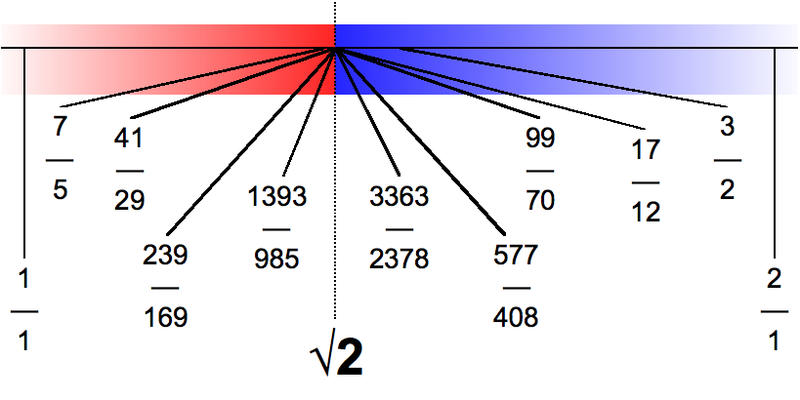
\includegraphics[scale=0.6]{img/Dedekind-cut.eps}
 %\captionsetup{labelformat=empty}
 \caption{Define $\sqrt{2}$ with Dedekind cut}
 \label{fig:Dedekind-cut}
\end{figure}

When apply Dedekind cut to all rational numbers, we can find that rationals are not continuous. For example, $A_1$ contains all rational numbers less than or equal to 2, and $A_2$ contains all rational numbers greater than 2, then this cut defines rational number 2. However for the negative example: the downwards $A_1$ contains all rational numbers that are negative, and the non-negative ones, but with their square less than or equal to 2; The upwards $A_2$ contains the rest rational numbers. We can find in this cut, there is no greatest number in the downwards, while there is no smallest number in the upwards too. It means there is a gap in rational numbers. When cut at this point, the knife will pass through. This cut actually defines a new number $\sqrt{2}$, and it is not a rational number, as shown in figure \ref{fig:Dedekind-cut}.

Dedekind came to the idea that every real number $r$ divides the rational numbers into two subsets, namely those greater than $r$ and those less than $r$. Dedekind's brilliant idea was to represent the real numbers by such divisions of the rationals. Every cut of a rationals defines a real number. The cut through a gap (no greatest in $A_1$, and no smallest in $A_2$) is an irrational number; the cut at a point ($A_1$ has the greatest, or $A_2$ has the smallest) is a rational number. And real numbers contain both rationals and irrationals. Hence Dedekind cut defines real numbers. Every point in the number line is a real number. It also gives the foundation of the continuity of real numbers.

From Hippasus found the irrational number, till Dedekind finally defined real numbers, It takes people two thousands years\footnote{In the same year of 1872, Weierstrass defined irrational numbers as limits of convergent series; Cantor also defined irrational numbers as convergent sequences of rational numbers. The theory of real numbers hence were established through these different paths.}. In the method of Dedekind cut, we always divide numbers into two finalized infinite parts, which are two infinite sets. This is the development and practice of actual infinity concept.

\subsection{Transfinite numbers and continuum hypothesis}
\index{power set}
On the way to find more numerous infinity, Cantor firstly considered power set. For a given set $A$, power set is the set of all possible subset of $A$. For example $A = \{a, b\}$, then its power set contains $\{\phi, \{a\}, \{b\}, \{a, b\}\}$, total four elements. For a set of 3 elements, its power set contains 8 subsets. Generally, for a set of $n$ elements, because every element can be select or skip when building a subset, the size of its power set is $2^n$. It's obvious that power set has a greater cardinality than the original finite set.

\index{Cantor's theorem}
Cantor proved in 1891, that even for any infinite set, the power set has a strict greater cardinality than the original set. This result is called {\em Cantor's theorem} nowadays. The proof is not hard, we put it in the appendix of this chapter. This theorem is the key to open the door to infinite of infinite world. Cantor introduced notation $\aleph_0$ for the cardinality of countable infinite set, like natural numbers. $\aleph$ is the first Hebrew letter. The cardinality of the power set for countable infinite set is $2^{\aleph_0}$. According to Cantor's theorem, $\aleph_0 < 2^{\aleph_0}$, on top of that, we can repeatedly use power set to generate greater and greater infinities.

\be
\aleph_0, 2^{\aleph_0}, 2^{2^{\aleph_0}}, ...
\ee

\subsubsection{Transfinite numbers}
\index{transfinite numbers}

康托尔把存在等级的无穷基数序列叫作超限基数。所以希尔伯特神奇旅馆中揭示的超限数计算法则就是$\aleph_0 + 1 = \aleph_0$, $\aleph_0 + k = \aleph_0 $, $\aleph_0 + \aleph_0 = \aleph_0$, ...

\index{序数}
除了用幂集来产生更高等级的无穷外,康托尔还发现了另外一种方法。为此,我们需要引入序数的归纳定义:

\begin{enumerate}
\item 0是序数;
\item 如果$a$是序数,则$a \cup \{a\}$是序数,记作$a + 1$,称作$a$的后继;
\item 如果$S$是序数的集合,也就是$S$的元素都是序数,则$\cup S$是序数;
\item 任何序数,都是通过上述1到3步获得的。
\end{enumerate}

根据这个定义,从0开始的前几个序数如下:

\[
\begin{array}{l}
0 \\
1 = 0 \cup \{0\} \\
2 = 1 \cup \{1\} = 0 \cup \{0\} \cup \{0 \cup \{0\}\} \\
3 = 2 \cup \{2\} = 1 \cup \{1\} \cup \{1 \cup \{1\}\} = ... \\
... \\
\end{array}
\]

这里$\cup S$称为集合$S$的广义并。它是由$S$的所有元素的元素组成的集合。根据序数定义的前两条,我们发现自然数0, 1, 2, 3, ..., n, ... 都是序数。令$\omega$是自然数集合,由于自然数都是序数,所以$\omega$也是一个序数的集合。我们考虑它的广义并:

\[
\cup \omega = \{0, 1, 2, ...\} = \omega
\]

根据序数的第三条定义,说明$\omega$也是一个序数,它是一个极限序数,并且是最小的无穷序数。我们把它添加到自然数的末尾就得到了一个新序列:

\[
0, 1, 2, ..., \omega
\]

从$\omega$开始,再次重复使用序数的第二条定义,又可以得到序数列:

\[
\omega + 1, \omega + 2, \omega + 3, ..., \omega + n, ...
\]

将上面两个序列合并到一起组成一个集合,记作$\omega \cdot 2$。不难发现其广义并$\cup \omega \cdot 2 = \omega \cdot 2$。所以$\omega \cdot 2$也是一个序数,并且是极限序数。从$\omega \cdot 2$开始,继续重复上述过程,我们就得到了无限伸展的无穷序数列:

\be
\begin{array}{l}
0, 1, 2, ..., n, ... \\
\omega, \omega + 1, \omega + 2, ..., \omega + n, ... \\
\omega \cdot 2, \omega \cdot 2 + 1, \omega \cdot 2 + 2, ..., \omega \cdot 2 + n, ... \\
...\\
\omega \cdot k, \omega \cdot k + 1, \omega \cdot k + 2, ..., \omega \cdot k + n, ... \\
... \\
\omega^2, \omega^2 + 1, \omega^2 + 2, ..., \omega^2 + n, ... \\
...\\
\omega^3, \omega^3 + 1, \omega^3 + 2, ..., \omega^3 + n, ... \\
...\\
\omega^\omega, \omega^\omega + 1, \omega^\omega + 2, ..., \omega^\omega + n, ... \\
...\\
\end{array}
\label{eq:countable-ordinal-nums}
\ee

除了第一行是自然数外,其它都是无穷序数,并且每行的第一个是极限序数。用这种方式得到的序数,已经远远超出人们所能想象的范围,把自然数扩展成一个无穷无尽的序数王国。但是,可以证明,这些序数都是可数序数,作为集合,竟然能够与自然数集构成一一对应。我们即将看到,还存在着不可数序数,甚至存在着一个比一个更大的无穷序数列。

我们列出的这些序数中,如果挑选一个作为可数集合的基数,用哪一个最好呢?自然会想到最小的一个极限序数$\omega$。于是这引出了基数的一般定义:

\index{基数}
\begin{definition}
设$a$是一个序数,如果对于任一序数$b$,当$b < a$时,有$b$的势小于$a$的势,则称序数$a$为基数。
\end{definition}

有这个定义,我们立即得出结论:所有自然数$n$都是基数,并且$\omega$是基数。序数$\omega$当作基数使用时,记作$\aleph_0$。即$\aleph_0 = \omega$,前面我们已经用$\aleph_0$表示可数集合的基数。

除了$\omega$外,序列(\ref{eq:countable-ordinal-nums})中其余的无穷序数都比$\omega$大,但其势却与$\omega$的势相等(都等于可数无穷)。所以根据定义,它们都不是基数。

为了获取更大的基数,为此我们将此前序列(\ref{eq:countable-ordinal-nums})中的所有序数汇集在一起组成一个集合,记作$\omega_1$。

\[
\omega_1 = \{ a | a \text{是序数,且} |a| \leq \aleph_0\}
\]

其中$|a|$表示$a$的势\footnote{严格来说,$A$的势应使用符号$\overline{\overline{A}}$,或$\#A, card(A), n(A)$。}。可以证明$\omega_1$是序数,并且是第一个不可数序数。然后我们仿照前面的方法,从$\omega_1$之后扩展无穷序数列:

\[
\omega_1, \omega_1 + 1, ..., \omega_1 \cdot 2, ..., \omega_1^2, ..., \omega_1^\omega, ...
\]

这里枚举的无穷序列都是等势的,其中最小的一个是$\omega_1$,它还满足基数的条件,这样我们就得到了第二个无穷基数$\aleph_1 = \omega_1$。仿照$\omega_1$的构造过程,我们可以再构造一个集合:

\[
\omega_2 = \{ a | a \text{是序数,且} |a| \leq \aleph_1\}
\]

这样就获得了第三个无穷基数$\aleph_2 = \omega_2$。继续进行下去,我们可以得到一系列无穷基数。概括来说,对任一序数$a$,当定义了无穷基数$\aleph_a$之后,我们可以再次构造集合:

\[
\omega_{a+1} = \{ b | b \text{是序数,且} |b| \leq \aleph_a\}
\]

由此得到比$\aleph_a$大的无穷基数$\aleph_{a+1} = \omega_{a+1}$。总之对于任一序数$a$,相应都有一个无穷基数$\aleph_a$,由此得到无穷基数组成的无穷序列:

\be
\aleph_0, \aleph_1, \aleph_2, ..., \aleph_n, ..., \aleph_{\omega}, ...
\ee

它们是从小到大排列的,并且相邻的两个阿列夫之间不再有其它的无穷基数。无穷序数和无穷基数也称为超限序数和超限基数,统称为超限数。这些越来越巨大的超限数最终归于何处呢?康托尔认为那将是上帝。

超限数一经面试,立即引发了激烈的反应。有人赞叹这是康托尔惊人的创举,开辟了前所未见的新视野。也有人认为超限数是“雾上之雾”,康托尔正在创造病态的数学。尽管存在巨大的争议,超限数是十九世纪最惊人的思想成就之一。

\subsubsection{连续统假设}
\index{连续统假设} \index{CH} \index{GCH}
康托尔发现了两种无穷基数序列,一个是幂集,另一个是超限基数:

\[
\aleph_0, 2^{\aleph_0}, 2^{2^{\aleph_0}}, ...
\]

和

\[
\aleph_0, \aleph_1, \aleph_2, ...
\]

根据上面的分析,我们知道$\aleph_1$是紧跟着可数无穷基数$\aleph_0$之后的下一个超限基数。然而根据幂集的性质,我们只知道$2^{\aleph_0}$比可数无穷基数$\aleph_0$大。但我们不知道它和$\aleph_1$的大小关系。康托尔猜测$2^{\aleph_0} = \aleph_1$,也就是在$\aleph_0$和$2^{\aleph_0}$之间不存在其它无限基数。$2^{\aleph_0}$是第一个比可数集大的超限基数。

康托尔在1847年证明了$2^{\aleph_0} = C$,也就是说,自然数的所有子集所具有的元素数正好等于实数集的元素数。因此康托尔的猜测等价于说在可数集$\aleph_0$与不可数集$C$之间不存在其它无限基数。由于通常称实数集为连续统,因此这一猜想被称为连续统假设,英文为:Continuum Hypothesis,简记为CH。

连续统假设还可以进一步推广。即考虑对于任一序数$a$,$2^{\aleph_a} = \aleph_{a+1}$是否成立。这一假设被称为广义连续统假设,简记为GCH。

康托尔在1878年的一篇论文提出了连续统假设。他一开始对证明这一猜想是比较乐观的。据说康托尔曾经说他已经成功解决了这一难题,并即将公布他的证明。但直到他1918年去世,也没有把证明公之于众。大概是发现了证明中的问题而未公开发表。康托尔晚年为此投入了大量的精力,但是长时间未能突破连续统假设,加之其它原因最终导致他陷入了抑郁,并在哈雷大学的精神病院中逝世。

1900年夏天,著名的数学家希尔伯特在巴黎召开的第二届国际数学家大会上,作了题为《数学问题》的演说。提出了23个未解决的问题,向二十世纪的数学家提出挑战。其中第一个问题就是“证明连续统假设”。可见他对这一问题的重视。

连续统问题是数学来源于几何、力学、和物理等方面现实问题的一个范例。希尔伯特认为,连续统问题来自外部世界,纯数学需要从外部世界汲取新材料,外部世界是数学的源泉。正因为连续统问题是数学中一个最基本的问题,或者说它是数学基础的问题,长期以来一直是数理逻辑和公理集合论的一个中心问题。一百多年来,虽然经过许多著名数学家的精心钻研。取得了一些重大进展,但还没有完全解决。1938年哥德尔证明了,从公理集合论的ZFC系统(策梅罗——弗兰克尔系统加上选择公理的简称,选择公理是说我们能从任一集合,包括无穷集合中选出若干元素。我们将在下一章详细介绍)推不出CH的否定。即连续统假设与ZFC系统是相容的。在哥德尔的结果之后,人们希望能够从ZF系统(ZF系统是不带有选择公理的集合论系统)内证明连续统假设。

1963年7月,美国的年轻数学家科恩创造了威力极大的力破法,解决了相反的问题,他证明了从ZFC推不出CH。这就说明了连续统假设和ZFC系统是相对独立的。有一则插曲说,科恩完成了证明后,并不能确信自己的证明(\cite{HanXueTao16},第280页)。他来到普林斯顿敲响了哥德尔的家门。当时的哥德尔正在同妄想症斗争,他仅仅打来了一条门缝,让科恩把证明塞进去。科恩则被关在了门外。两天后,哥德尔邀请科恩进屋喝茶,大师终于认可了他的证明。

综合哥德尔和科恩的结果,也就是说连续统假设在ZFC系统中是不可判定的。我们在下一章会深入介绍不可判定性。连续统假设与ZF系统的公理无关。类似的结论还发生在集合论中的选择公里上。哥德尔和科恩的结论同时也说明,选择公理在ZF系统中是不可判定的。这说明在ZF公理集合论系统中,承认选择公理可以得到一种数学;否定选择公理可以得到另一种数学。两者都是无矛盾的。同样,加上选择公理后,承认或者否定连续统假设也都可以各自发展出无矛盾的数学。这就是100多年来人们在选择公理与连续统假设的研究中获得的主要成果\cite{GCH}。

\section{无穷与艺术}

\begin{figure}[htbp]
%\begin{wrapfigure}{R}{0.5\textwidth}
 \centering
 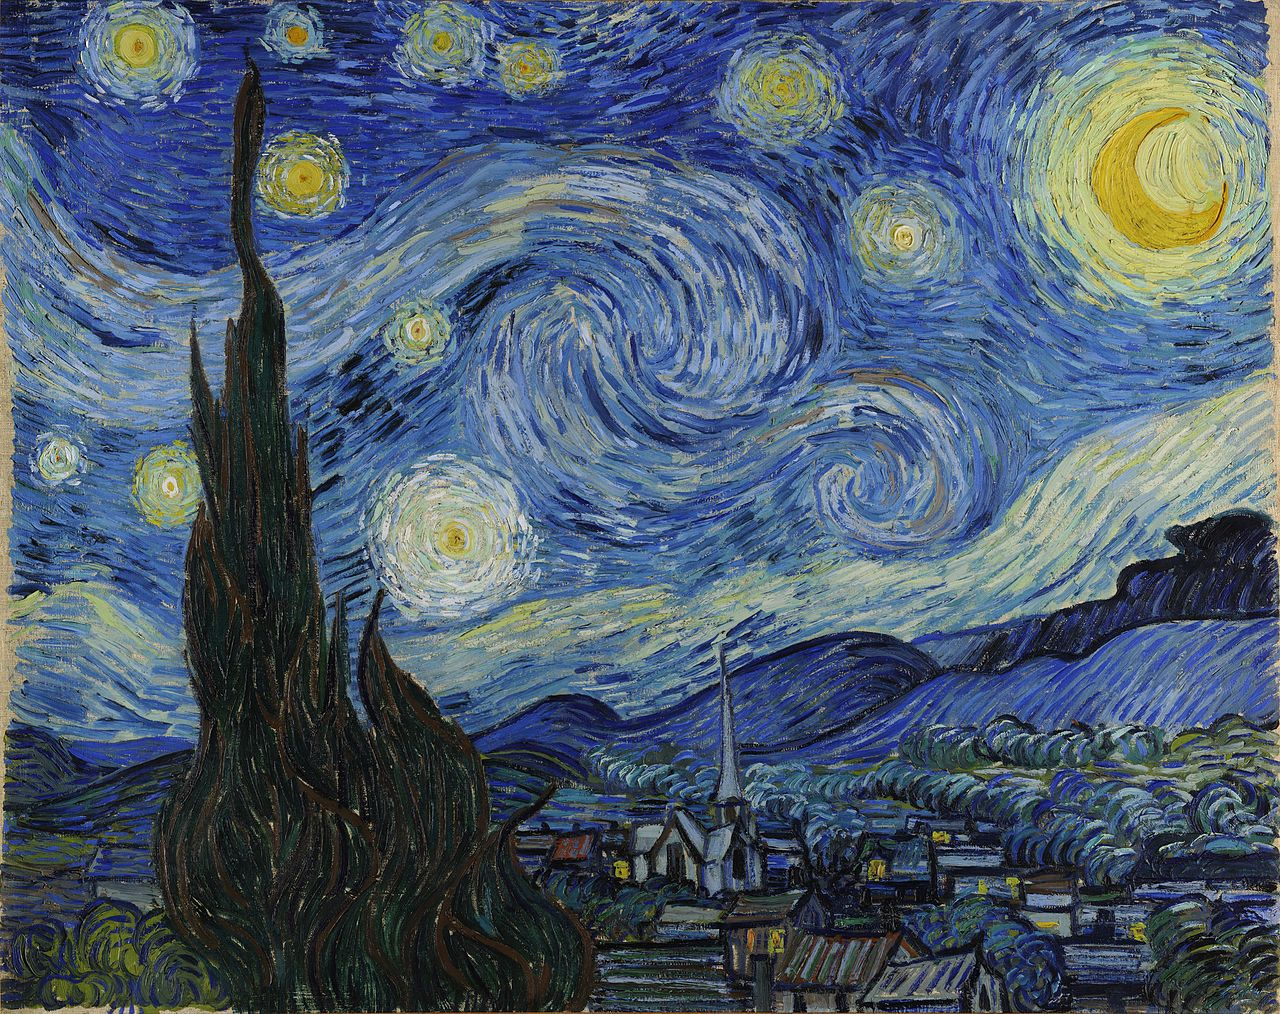
\includegraphics[scale=0.15]{img/starry-night.eps}
 \captionsetup{labelformat=empty}
 \caption{[荷]梵高《星空》1889,原作收藏于纽约现代艺术博物馆}
 \label{fig:starry-night}
%\end{wrapfigure}
\end{figure}

伴随着对无穷的思考与探索,也不断催生了关于无穷的艺术创作。人们仰视浩瀚苍穹,远眺无垠的大海,感叹自然的神秘和伟大。

在无数描绘广袤天空的作品中,荷兰后印象派艺术大师梵·高创作的《星空》可谓让人印象深刻。在这幅画中,梵高用夸张的手法,生动地描绘了充满运动和变化的星空。 整个画面被一股汹涌、动荡的蓝绿色激流所吞噬,旋转、躁动、卷曲的星云使夜空变得异常活跃,脱离现实的景象反映出梵·高躁动不安的情感和疯狂的幻觉世界。这幅画创作于1889年,当时梵·高正在阿尔勒圣雷米的一家精神病院治疗,在那驻留了108天。在入住精神病院期间,梵高创作了大量的绘画作品,共计一百五十多幅油画和一百多幅素描。而作品《星空》所描述的风景也正是精神病院所在地圣雷米。

\begin{figure}[htbp]
%\begin{wrapfigure}{R}{0.5\textwidth}
 \centering
 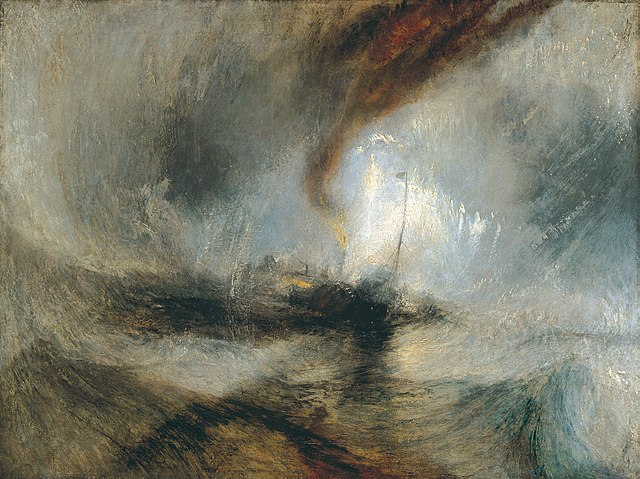
\includegraphics[scale=0.3]{img/Turner-Snow-Storm.eps}
 \captionsetup{labelformat=empty}
 \caption{透纳笔下的大海和风暴,1842。原作藏于英国泰特美术馆}
 \label{fig:Turner-Snow-Storm}
%\end{wrapfigure}
\end{figure}

英国画家透纳,在创作《暴风雪:汽船驶离港口》时,为了充分体验大海无边的威力,他让水手把自己捆在船桅上。他后来写道:“为了观察大海,我让水手们把我捆在船桅上。我那样过了四个小时,没指望能活下来。”然而,评论家们却对这幅画表示失望和怀疑,因为在这幅画中,形体和戏剧性的场面都消失了。透纳解释说,他画这幅画是为了告诉自己和别人,在惊涛骇浪的海上,暴风雪是什么样子。虽然描画的是在漩涡风暴中航行的船,但是所呈现的却是船只与风暴融为一体的画面。透纳大胆地以抽象手法表现船的形式,自由运用色彩,成功的表现出“风暴的气氛”。透纳因此被称为印象派的先驱。

对无穷的思考很快脱离了自然界中的具体事物,而上升到哲学和宗教。在托勒密的宇宙模型中,行星是嵌套在一起的同心球,最外层存在一个有界的恒星天球。到了中世纪,基督教在很大程度上吸收了亚里士多德和托勒密的学说,认为上帝创造的地球是宇宙的中心,而恒星天球是有界的。

\begin{figure}[htbp]
 \centering
 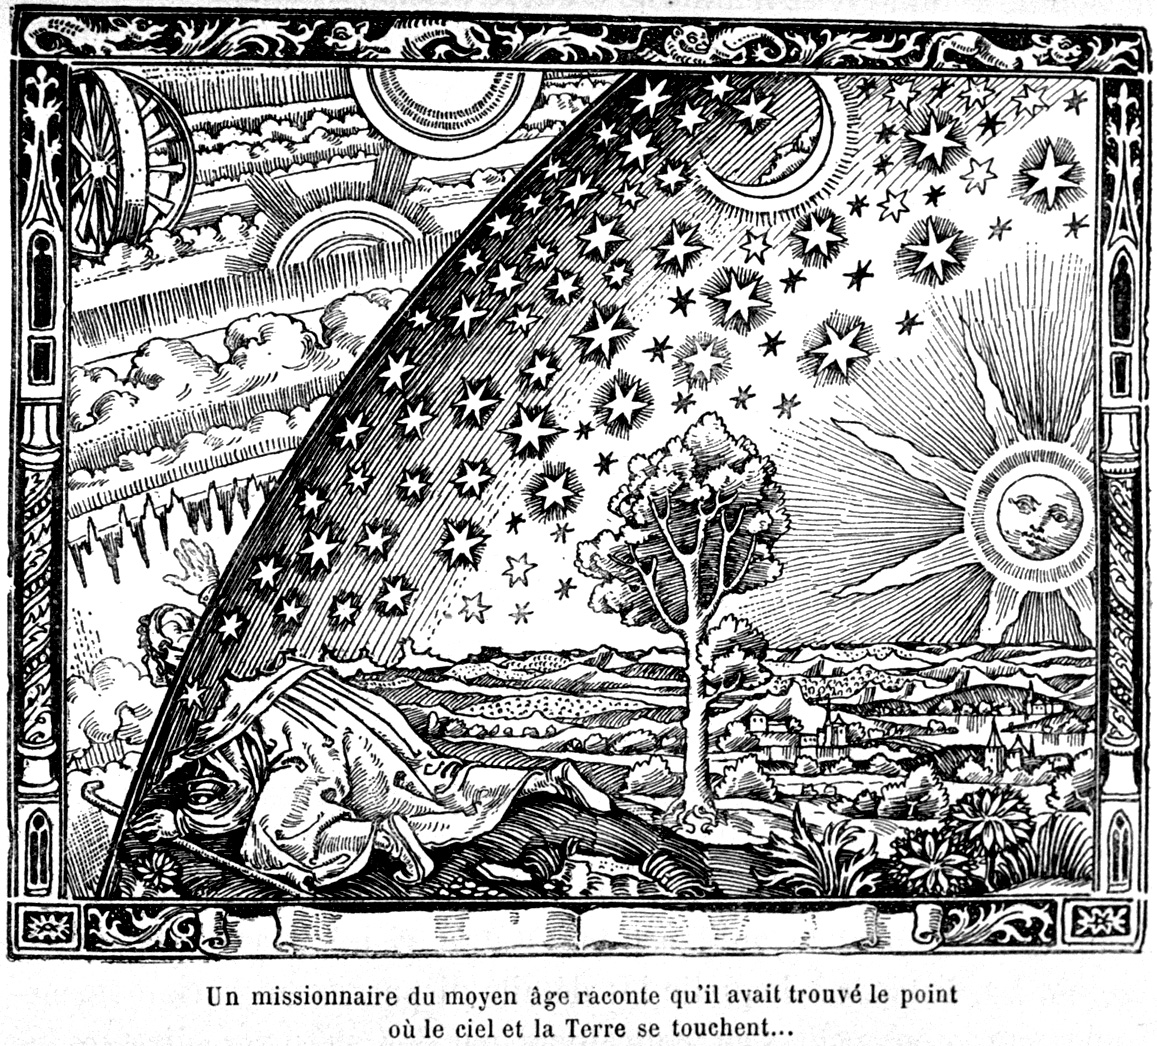
\includegraphics[scale=0.3]{img/Flammarion.eps}
 \captionsetup{labelformat=empty}
 \caption{1888年在巴黎出版的《弗拉马利翁》木刻版画,第163页,作者为无名氏}
 \label{fig:Flamarion-woodcut}
\end{figure}

%% Camille Flammarion, L'Atmosphere: Météorologie Populaire (Paris, 1888), p. 163.

%% The Flammarion Woodcut is an enigmatic woodcut by an unknown artist. It is referred to as the Flammarion Woodcut because its first documented appearance is in page 163 of Camille Flammarion's L'atmosphère: météorologie populaire (Paris, 1888), a work on meteorology for a general audience. The woodcut depicts a man peering through the Earth's atmosphere as if it were a curtain to look at the inner workings of the universe.

%% The original caption bellow the picture translated to: "A medieval missionary (Bruno) tells that he has found the point where heaven and Earth meet...".

1888年在巴黎出版的一幅木刻版画反映了当时人们对于有穷世界边沿的思考。一个人如果站在天球的边沿,是否可以伸出自己的手臂或者举起一根手杖?如果不可以,这显然是难以理解的,如果可以,那么处于物质世界外围的空间是什么?这就是宇宙边缘悖论。为了解决这个难题,中世纪的基督教重塑了亚里士多德的学说,提出了一种渐进边缘理论。还有人为,如果在宇宙的边缘向外抛出一支矛,就会推动宇宙扩大。物质世界是有界的,但界被无尽的虚空包围。

文艺复兴时期,数学逐渐被当时艺术大师们引入到作品中。达芬奇不仅深谙解刨和透视,还有意识地在在作品中使用引发美感的比例。这一时期的德国画家丢勒仔细研究了人体的各种比例,甚至利用坐标格点来描述透视的关系。丢勒的《量度四书》既介绍了绘画理论,也对几何原理和透视原理进行了研究。随后开普勒和笛沙格独立发展出了摄影几何中的无穷远点概念。笛沙格概括消失点的用途,纳入无穷远时的情形,发展出建构透视图的另一种方法。他让平行线确实平行的欧氏几何成为所有可能的几何系统都会有的特例。

\index{非欧几何}
真正从本质上改变了艺术家的视角,使得人们能够直接表现无穷要从非欧几何的诞生说起。长期以来,欧几里得几何被人们认为是完美的公理系统和演绎推理的典范。但是追求尽善尽美的数学家对于欧几里得第五公设颇有微词。前几条公设简单直观,符合直觉,例如说两点之间能够画一条直线,所有直角都相等。而第五公设描述却比较复杂。它说如果某条直线与两直线相交,且同侧两个内角和小于两个直角,那么两条直线无限延长后就会在该侧相交。第五公设也叫作平行公设,它等价于说,在平面内过直线外一点有且仅有一条平行线。人们感觉第五公设能从前面四条公设里推导出,并且实际上欧几里得在《几何原本》前面相当大的部分也都没有使用第五公设。在其后的两千多年里,很多人试图证明第五公设,但都失败了。于是意大利数学家撒凯里(Saccheri)尝试用反证法来证明,他假定第五公设不成立,然后导出一整套几何系统和奇怪的结论,接下来他宣称这些结果太过荒谬,从而说明第五公设是必定是正确的。

19世纪,德国数学家高斯、俄国数学家罗巴切夫斯基、匈牙利数学家波尔约等人各自独立地认识到这种证明是不可能的。也就是说,平行公理是独立于其他公理的,并且可以用不同的“平行公理”来替代它。高斯关于非欧几何的信件和笔记在他生前一直没有公开发表,只是在他1885年去世后出版时才引起人们的注意。罗巴切夫斯基和波尔约分别在1830年前后发表了他们关于非欧几何的理论。在这种几何里,罗巴切夫斯基平行公理替代了欧几里得平行公理,即在一个平面上,过已知直线外一点至少有两条直线与该直线不相交。由此可演绎出一系列全无矛盾的结论,并且可以得出三角形的内角和小于两直角。罗氏几何中有许多不同于欧氏几何的定理。

继罗氏几何后,德国数学家黎曼在1854年又提出了既不是欧氏几何也不是罗氏几何的新的非欧几何。这种几何采用如下公理替代欧几里得平行公理:同一平面上的任何两直线一定相交。同时,还对欧氏几何的其他公理做了部分改动。在这种几何里,三角形的内角和大于两直角。人们把这种几何称为椭圆几何。

直到1866年,意大利数学家贝尔特拉米在他出版的《非欧几何解释的尝试》中,证明了非欧平面几何可以局部地在欧氏空间中实现。1871年,德国数学家克莱因认识到从射影几何中可以推导度量几何,并建立了非欧几何模型。这样,非欧几何的相容性问题就归结为欧氏几何的相容性问题,由此非欧几何得到了普遍的承认。

%\begin{wrapfigure}{L}{0.4\textwidth}
\begin{figure}[htbp]
 \centering
 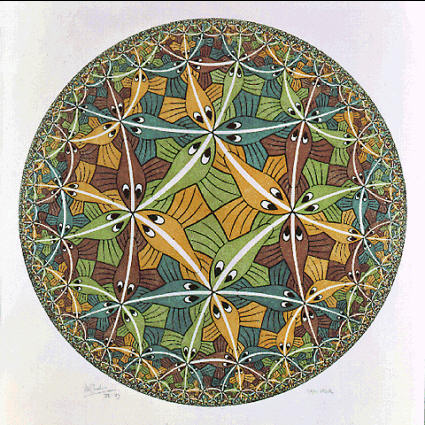
\includegraphics[scale=1.0]{img/circle-limit-III-1959.eps}
 \captionsetup{labelformat=empty}
 \caption{埃舍尔《圆极限$\cdot$3》1959}
 \label{fig:circle-limit-3}
\end{figure}
%\end{wrapfigure}

非欧几何向我们揭示这样一种可能性,即无穷的空间可能是有界的。法国数学家庞加莱在他的科普读物《科学与假设》中介绍了这样一种有趣的世界。整个世界被一个大小有限的球包围起来。中心的温度很高,随着远离中心,温度成比例地减小。当接近包围这这个世界的球面时,温度降到绝对零度。如果大球的半径是$R$,某点到球心的距离是$r$,则温度与$R^2 - r^2$成比例。这个世界中,由于热胀冷缩,物体的大小和温度成比例,越接近世界的边沿,物体越小。于是就出现这样的一个奇观,当这个世界的居民接近球面时,温度越来越低,他们越来越小,步伐也越来越小,他们永远也到不了世界的边沿,尽管这个世界是有限的。庞加莱描述的这个世界,实际上起作用的几何是一种称为双曲几何的非欧几里得几何学。

荷兰画家埃舍尔受到庞加莱的启发,创作了多个艺术作品来描述这种有限但无穷的世界。这一系列作品被命名为圆极限系列。不管是天使、魔鬼、还是游动的鱼,都在接近圆盘的边缘时变小,从而永远无法到达这个有界但无穷的边沿。

不仅是艺术,在音乐中也有对无穷的思索和表现。1747年5月,巴赫访问了波茨坦宫廷圣苏西宫。巴赫到了圣苏西宫后,腓特烈大帝向他展示了刚刚引进的吉尔博曼钢琴。宫廷音乐会上腓特烈大帝给了巴赫一个音乐主题,老巴赫当场即兴对其进行了一个三声部的赋格变奏。这是事前毫无演练的即兴演奏。这不仅使大帝十分满意,在场众人也无不瞠目结舌。巴赫本人觉得这首曲子的主题非常美丽,于是打算将来写成一首赋格曲,以供出版。回到莱比锡后,巴赫重新对国王主题进行变奏创作,将整个曲子按两首赋格曲,四乐章三重奏鸣曲和十首卡农的构成完成了整个曲子。巴赫在献词上所署名的时间正好是7月7日。这就是巴赫的经典名作《音乐的奉献》,乐曲编号BWV1079。在其中有一首极不寻常的卡农,只标着“Canon per Tonos”这三个词。翻译过来的意思是经由种种调性的卡农。后人称之为“无穷升高的卡农”。侯世达在《哥德尔、埃舍尔、巴赫——集异璧之大成》一书中写到:

\begin{figure}[htbp]
%\begin{wrapfigure}{R}{0.4\textwidth}
 \centering
 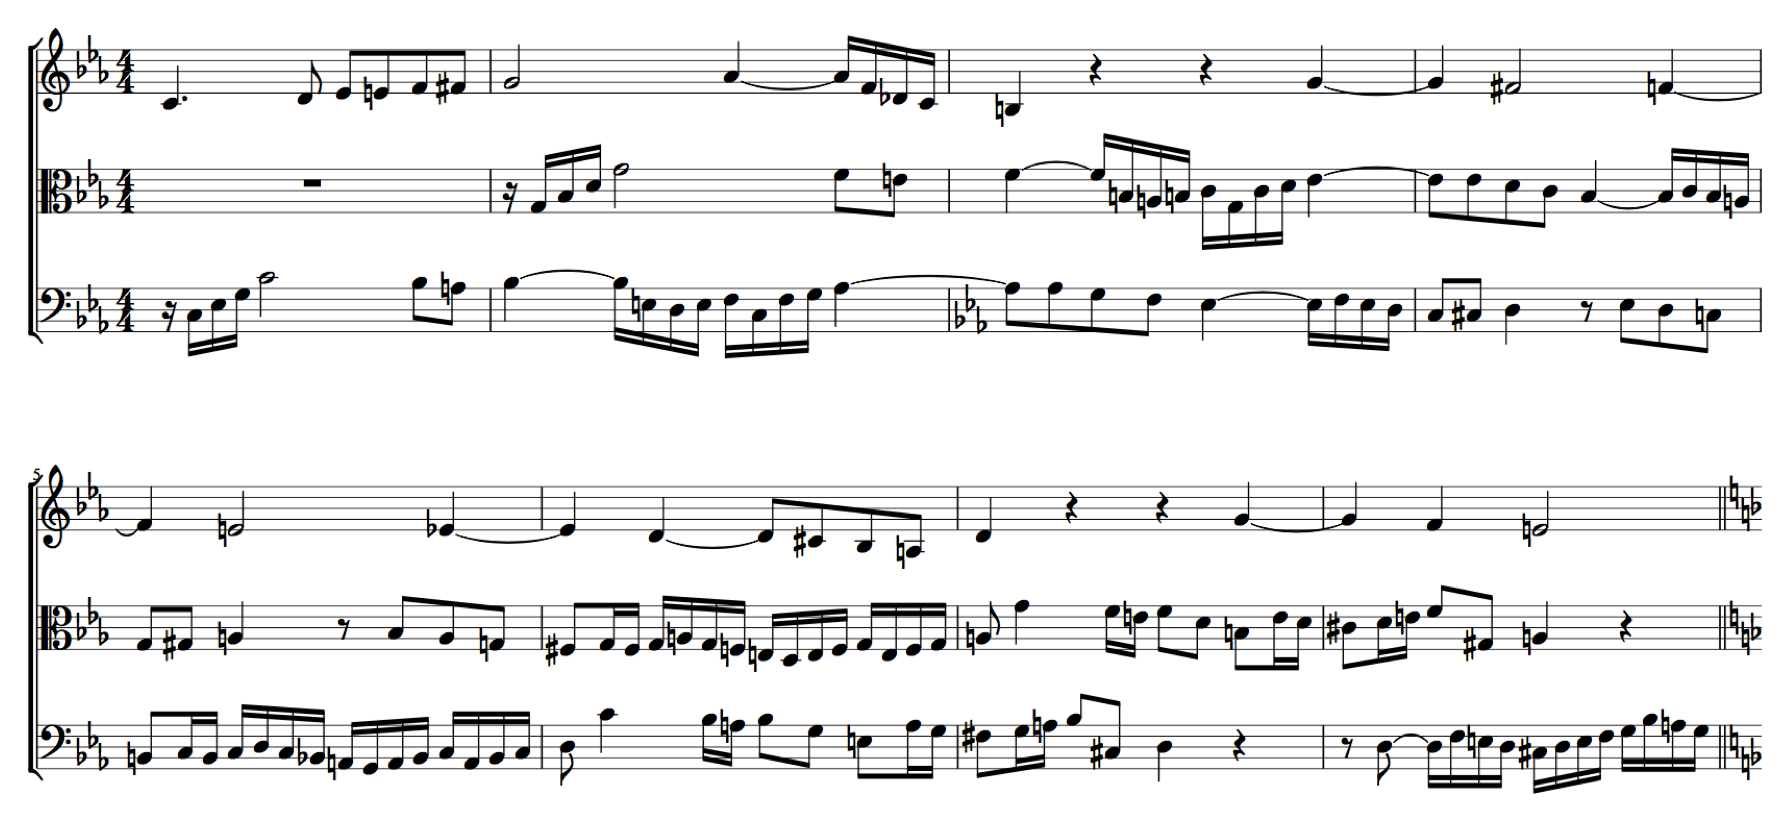
\includegraphics[scale=0.3]{img/canon-endless.eps}
 \captionsetup{labelformat=empty}
 \caption{巴赫创作的无穷升高的卡农的曲谱局部}
 \label{fig:canon-endless}
%\end{wrapfigure}
\end{figure}

它有三个声部,最高声部是国王主题的一个变奏,下面两个声部则提供了一个建立在第二主题之上的卡农化的和声。这两个声部中较低的那个声部用C小调奏出主题,而较高的那个则在差五度之上奏出同一主题。特殊之处在于,当它结束时——或者不如说似乎要结束时——已不再是C小调而是D小调了。巴赫在听众的鼻子底下转了调。而且这一结构使得这一“结尾”很通顺地与开头联接起来。这样可以重复这一过程并在E调上回到开头。这些连续的变调带着听众不断上升到越来越远的调区,因此听了几段之后,听众会以为他要无休止地远离开始的调子了。然而在整整六次这样的变调之后,原来的C小调又魔术般地恢复了!所有的声音都恰好比原来高八度。在这里整部曲子可以以符合音乐规则的方式终止。人们猜想,这里就是巴赫的意图。但巴赫很明确地留下了一个暗示,说这一过程可以无休止地进行下去。也许这就是为什么他在边上写下了“转调升高,国王的荣耀也升高。”\cite{GEB}

\begin{Exercise}
\Question{在两个镜子中间点燃一支蜡烛,你看到了什么?这是潜无穷还是实无穷?}
\end{Exercise}

\section{附录:例子代码}

使用流定义自然数潜无穷,并取出前15个自然数。Java语言1.8中的例子:

\lstset{frame=single, language=Java}
\begin{lstlisting}
IntStream.iterate(1, i -> i + 1);

IntStream.iterate(1, i -> i + 1)
        .limit(15).forEach(System.out::println);
\end{lstlisting}

Python语言版本3中的例子:

\lstset{frame=single, language=Python}
\begin{lstlisting}
def naturals():
    yield 0
    for n in naturals():
        yield n + 1
\end{lstlisting}

Haskell语言中使用递归定义自然数潜无穷:

\lstset{frame=single, language=Haskell}
\begin{lstlisting}
nat = 1 : (map (+1) nat)

take 15 nat
\end{lstlisting}

Haskell语言中使用递归定义斐波那契数列潜无穷,以及计算第1500个斐波那契数。

\lstset{frame=single, language=Haskell}
\begin{lstlisting}
fib = 0 : 1 : zipWith (+) fib (tail fib)

take 15 fib
[0,1,1,2,3,5,8,13,21,34,55,89,144,233,377]

fib !! 1500
13551125668563101951636936867148408377786010712418497242133543153221487310
87352875061225935403571726530037377881434732025769925708235655004534991410
29242495959974839822286992875272419318113250950996424476212422002092544399
20196960465321438498305345893378932585393381539093549479296194800838145996
187122583354898000
\end{lstlisting}

Haskell语言中使用余代数定义素数的潜无穷流

\lstset{frame=single, language=Haskell}
\begin{lstlisting}
data StreamF e a = StreamF e a
data Stream e = Stream e (Stream e)

takeStream 0 _ = []
takeStream n (Stream e s) = e : takeStream (n - 1) s

era (p:ns) = StreamF p (filter (p `notdiv`) ns)
  where notdiv p n = n `mod` p /= 0

primes = ana era [2..]

takeStream 15 primes
[2,3,5,7,11,13,17,19,23,29,31,37,41,43,47]
\end{lstlisting}

\section{附录:康托尔定理的证明}

\begin{theorem}
\textbf{康托尔定理}:对于任意集合都有$|S| < |2^S|$,其中$|S|$表示集合$S$的势,$2^S$表示$S$的幂集,即$S$的所有子集组成的集合。
\end{theorem}

\begin{proof}
我们分两步证明。首先证明$|S| \leq |2^S|$。对于任一$x$,令$f(x) = \{x\}$,也就是仅含有$x$唯一元素的集合。对于不同的元素$x_1 \neq x_2$,自然有$\{x_1\} \neq \{x_2\}$,即$f(x_1) \neq f(x_2)$。从而映射$S \arrowto{f} 2^S$是一单射。因此有
\[
  |S| \leq |2^S|
\]

第二步,我们证明$|S| \neq |2^S|$。采用反证法,假设等号成立。则存在一一映射$S \arrowto{\phi} 2^S$,使得对任一$x \in S$,都有$\phi(x) \in 2^S$。即$\phi(x)$是$S$的某个子集,所以$\phi(x) \subseteq S$。现在要问:$x$是否属于$\phi(x)$?有两种可能:一种是$x \in \phi(x)$,也可能是$x \notin \phi(x)$。我们把所有$x$不属于$\phi(x)$的元素放在一起构造一个新集合$S_0$:

\be
S_0 = \{ x | x \in S, \text{并且} x \notin \phi(x)\}
\label{eq:def-s0}
\ee

显然$S_0$是$S$的子集,即$S_0 \subseteq S$,因此$S_0 \in 2^S$。由于$\phi$是一一映射,所以必然存在一个$x_0$,使得$\phi(x_0) = S_0$。根据逻辑中的排中律,要么$x_0 \in S_0$,要么$x_0 \notin S_0$,二者必居其一,且仅有一个成立。

接下来分情况讨论。如果$x_0 \in S_0$成立,根据式(\ref{eq:def-s0})中$S_0$的定义,应该有$x_0 \notin \phi(x_0)$,由于$\phi(x_0) = S_0$,所以$x_0 \notin S_0$。

如果$x_0 \notin S_0$,因为$S_0 = \phi(x_0)$,所以得到$x_0 \notin \phi(x_0)$。这样根据$S_0$的定义(\ref{eq:def-s0}),又应该有$x_0 \in S_0$。

这样不论$x_0$是否属于$S_0$,都导致矛盾。这说明我们最初的假设$S$到$2^S$间存在一一映射是错误的。所以不等式$|S| \neq |2^S|$成立。

由这两步的结果:$|S| \leq |2^S|$,并且$|S| \neq |2^S|$,我们得到了康托尔定理的结论:

\[
  |S| < |2^S|
\]
\end{proof}

证明的第二部分,不由让我们联想起了著名的罗素悖论:令$S$为所有不属于自己的集合构成的集合,问$S$是否属于自己?我们将在下一章讲述罗素悖论和哥德尔不完全性定理。

% Mathematicians aren't satisfied because they know there are no solutions up to four million or four billion, they really want to know that there are no solutions up to infinity. -- Andrew Wiles

\section{附录:巴赫《音乐的奉献》无限上升的卡农}

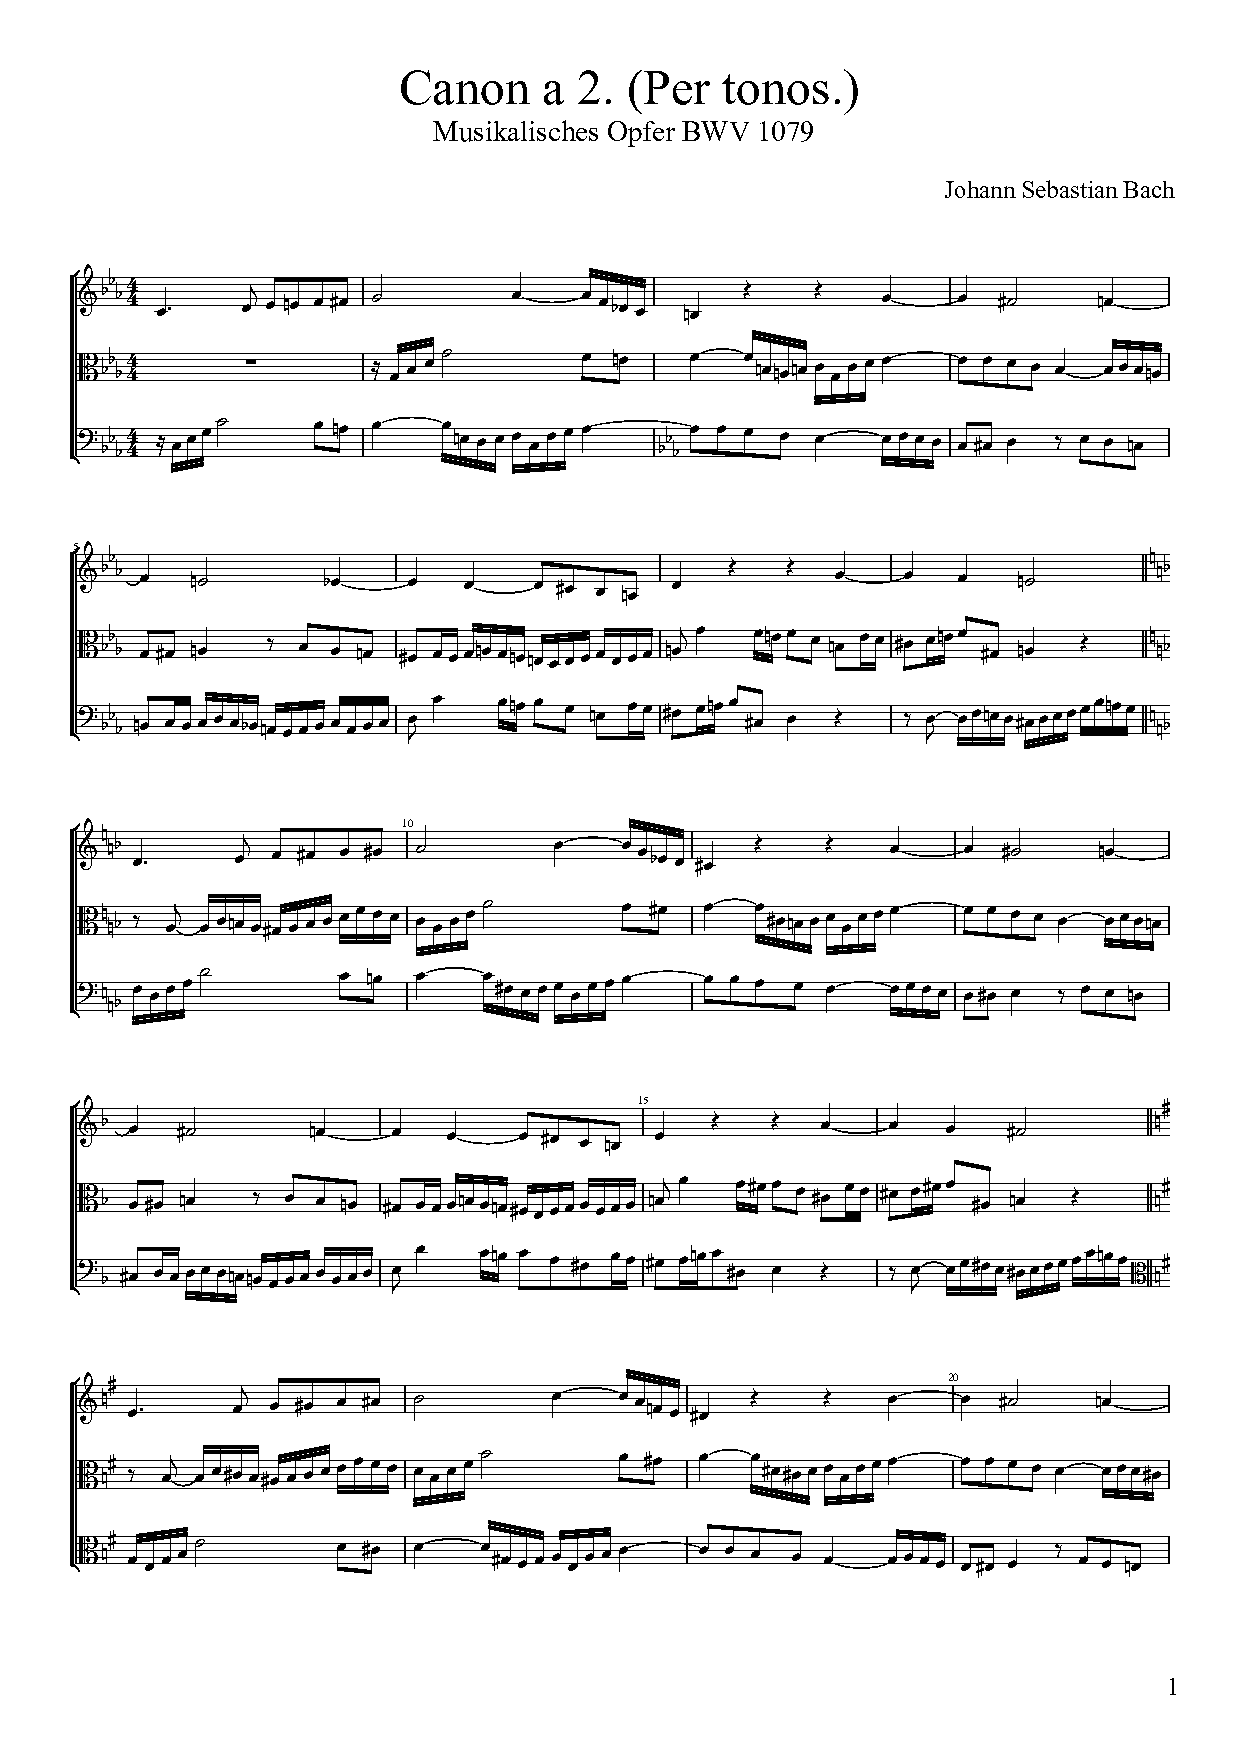
\includepdf[pages=-,
nup=2x2
, scale=0.85
%,fitpaper=true
]{img/bwv1079-canon-per-tonos.pdf}

\ifx\wholebook\relax \else
\begin{thebibliography}{99}

\bibitem{De-linfini-2018}
[法] 让-皮埃尔$\cdot$卢米涅,马克$\cdot$拉雪茨-雷 著,孙展 译. 从无穷开始——科学的困惑与疆界. 人民邮电出版社. 2018. ISBN: 9787115479198

\bibitem{Noguchi2007}
[日] 野口哲也 著,刘慧 韩丽红 译. 数学原来可以这样学. 湖南人民出版社. 2014. ISBN: 9787556100897
% Tetsunori Noguchi. SUGAKUTEKI SENSE GA MINITUKU RENSHUCHO.

\bibitem{Wikipedia-Googol}
Wikipedia. ``Googol''. \url{https://en.wikipedia.org/wiki/Googol}

\bibitem{Wikipedia-Zeno}
Wikipedia. ``Zeno's Paradoxes''. \url{https://en.wikipedia.org/wiki/Zeno's_paradoxes}

\bibitem{HanXueTao16}
韩雪涛 ``数学悖论与三次数学危机''. 人民邮电出版社. 2016, ISBN: 9787115430434

\bibitem{Elements}
[古希腊] 欧几里得 著,兰纪正 朱恩宽 译,梁宗巨 张毓新 徐伯谦 校订 ``几何原本''. 译林出版社. 2014, ISBN: 9787544750066

\bibitem{M-Kline-2007}
[美] M$\cdot$克莱因 著 李宏魁 译 ``数学:确定性的丧失'' 湖南科学技术出版社,2007年4月 ISBN: 978-7-5357-1857-0
% Morris Kline ``Mathematics: The Loss of Certainty''. Oxford University Press, 1980.

\bibitem{Stepanov}
Stepanov and Rose. ``数学与泛型编程''. 爱飞翔译,机械工业出版社。ISBN: 978-7-111-57658-7. 2017.

\bibitem{Calvin-Clawson-1994}
Calvin C Clawson. ``The Mathematical Traveler, Exploring the Grand History of Numbers''. Springer. 1994, ISBN: 9780306446450

\bibitem{GEB}
[美]候世达 ``哥德尔、埃舍尔、巴赫——集异壁之大成''. 商务印书馆 1996. ISBN: 978-7-100-01323-9

\bibitem{GCH}
张锦文,王雪生 ``连续统假设''. 世界数学名题欣赏丛书。辽宁教育出版社 1988. ISBN: 7-5382-0436-9/G$\cdot$445

\bibitem{Courant1969}
Richard Courant, Herbert Robbins , Reviewed by Ian Stewart. ``What Is Mathematics? An Elementary Approach to Ideas and Methods 2nd Edition''. Oxford University Press,  1996, ISBN: 978-0195105193.

\bibitem{Poincare1}
[法]彭加勒 著,李醒民 译 ``科学与假设'' 商务印书馆. 2006. ISBN: 978-7-100-04796-8

\end{thebibliography}

\expandafter\enddocument
%\end{document}

\fi
